\documentclass[11pt,letterpaper]{article}

% 1. IDIOMA Y CARACTERES
\usepackage[utf8]{inputenc}
\usepackage[T1]{fontenc}
\usepackage[spanish, es-nodecimaldot, es-noquoting]{babel}
\usepackage{csquotes}
\usepackage{mathpazo}          % Palatino para texto y matemáticas
\usepackage{textcomp}
\usepackage{microtype}

% 2. GEOMETRÍA
\usepackage[margin=2.2cm, headheight=14pt]{geometry}

% 3. ESPACIADO  (más aire: interlineado 1.15 y separación entre párrafos)
\linespread{1.15}
\setlength{\parskip}{0.72em}
\setlength{\parindent}{0pt}
% Empaquetado de floats: menos espacio en blanco forzado
\renewcommand{\topfraction}{0.92}
\renewcommand{\bottomfraction}{0.85}
\renewcommand{\textfraction}{0.07}
\renewcommand{\floatpagefraction}{0.78}
\setcounter{topnumber}{3}
\setcounter{totalnumber}{5}

% 4. MATEMÁTICAS
\usepackage{amsmath,amssymb}

% 5. TABLAS Y GRÁFICOS
\usepackage{booktabs}
\usepackage{array}
\usepackage{colortbl}
\usepackage{xcolor}
\usepackage{graphicx}
\usepackage{float}
\usepackage{pifont}
\usepackage{multirow}
\usepackage{caption}
\captionsetup{font=small,labelfont={bf,color=headerblue}}

% LISTADOS DE CÓDIGO
\usepackage{listings}
\lstdefinestyle{vp}{
    language=Python,
    basicstyle=\ttfamily\scriptsize,
    keywordstyle=\color{headerblue}\bfseries,
    commentstyle=\color{sectiongreen!80!black}\itshape,
    stringstyle=\color{alertred},
    numbers=none, frame=single, rulecolor=\color{gray!45},
    backgroundcolor=\color{gray!6}, breaklines=true, showstringspaces=false,
    columns=fullflexible, keepspaces=true, xleftmargin=6pt, framexleftmargin=6pt,
    aboveskip=6pt, belowskip=4pt,
}
\lstset{style=vp}

% Etiquetas de flotantes en español: "Tabla" (no "Cuadro") y "Listado" (no "Listing")
\addto\captionsspanish{%
  \renewcommand{\tablename}{Tabla}%
  \renewcommand{\listtablename}{\'Indice de tablas}%
}
\renewcommand{\lstlistingname}{Listado}

% 6. CAJAS
\usepackage{tcolorbox}
\tcbuselibrary{skins,breakable}

% 7. ENCABEZADOS
\usepackage{fancyhdr}
\pagestyle{fancy}
\fancyhf{}
\fancyhead[L]{\small\textsc{Reporte Final \textcolor{uacjgray}{\normalfont\textbullet} Optimización Inteligente}}
\fancyhead[R]{\small\textsc{Visa Predict AI \textcolor{uacjgray}{\normalfont\textbullet} MOHHO}}
\fancyfoot[C]{\thepage}
\renewcommand{\headrulewidth}{0.4pt}

% 8. HIPERVÍNCULOS
\usepackage{hyperref}
\hypersetup{colorlinks=true, linkcolor=blue!60!black, urlcolor=blue!60!black, citecolor=blue!60!black}

% 9. COLORES
\definecolor{headerblue}{HTML}{003CA6}
\definecolor{uacjyellow}{HTML}{FFD600}
\definecolor{sectiongreen}{HTML}{27AE60}
\definecolor{formulabg}{HTML}{F1F8E9}
\definecolor{formulaborder}{HTML}{DCEDC8}
\definecolor{restrictionbg}{HTML}{FFF3E0}
\definecolor{restrictionborder}{HTML}{FF9800}
\definecolor{deliverbg}{HTML}{E3F2FD}
\definecolor{tablehead}{HTML}{2C3E50}
\definecolor{uacjgray}{HTML}{555559}
\definecolor{alertred}{HTML}{B41E1E}
\definecolor{answerbg}{HTML}{E8F5E9}
\definecolor{answerborder}{HTML}{2E7D32}
\definecolor{examplebg}{HTML}{FFF8E1}
\definecolor{exampleborder}{HTML}{F9A825}
\definecolor{shotframe}{HTML}{1B2430}

% 10. CAJAS TCOLORBOX
\newtcolorbox{formulabox}{colback=formulabg,colframe=formulaborder,arc=4pt,boxrule=0.8pt,left=8pt,right=8pt,top=8pt,bottom=8pt}
\newtcolorbox{notebox}[1][]{colback=deliverbg,colframe=headerblue!40,borderline west={4pt}{0pt}{headerblue},arc=2pt,boxrule=0.5pt,left=10pt,right=10pt,top=8pt,bottom=8pt,#1}
\newtcolorbox{resultbox}[1][]{colback=formulabg,colframe=sectiongreen!60,borderline west={4pt}{0pt}{sectiongreen},arc=2pt,boxrule=0.5pt,left=10pt,right=10pt,top=8pt,bottom=8pt,#1}
\newtcolorbox{yellowbox}[1][]{colback=uacjyellow!10,colframe=uacjyellow!50,borderline west={4pt}{0pt}{uacjyellow},arc=2pt,boxrule=0.5pt,left=10pt,right=10pt,top=8pt,bottom=8pt,#1}
\newtcolorbox{answerbox}[1][]{colback=answerbg,colframe=answerborder,borderline west={4pt}{0pt}{answerborder},arc=2pt,boxrule=0.5pt,left=10pt,right=10pt,top=8pt,bottom=8pt,#1}
\newtcolorbox{examplebox}[1][]{colback=examplebg,colframe=exampleborder,borderline west={4pt}{0pt}{exampleborder},arc=2pt,boxrule=0.5pt,left=10pt,right=10pt,top=8pt,bottom=8pt,#1}
\newtcolorbox{restrictionbox}[1][]{colback=restrictionbg,colframe=restrictionborder,borderline west={3pt}{0pt}{restrictionborder},arc=2pt,boxrule=0.5pt,left=10pt,right=10pt,top=8pt,bottom=8pt,#1}

% Marco para capturas de pantalla (estética "presentación")
\setlength{\fboxsep}{0pt}
\newcommand{\shot}[2][\linewidth]{\fcolorbox{shotframe}{shotframe}{\includegraphics[width=#1]{#2}}}
% Celda de cuadrícula 2-up: imagen enmarcada + etiqueta
\newcommand{\galshot}[2]{\begin{minipage}[t]{0.315\textwidth}\centering\shot[\dimexpr\linewidth-2\fboxrule\relax]{#1}\\[1pt]{\scriptsize\color{headerblue}#2}\end{minipage}}

% 11. SECCIONES CON LÍNEA DORADA
\usepackage{titlesec}
\titleformat{\section}{\Large\bfseries\color{headerblue}}{\thesection.}{0.5em}{}[\vspace{-0.5em}{\color{uacjyellow}\rule{5pt}{0pt}\rule[0.3ex]{0.4\linewidth}{2pt}}]
\titleformat{\subsection}{\large\bfseries\color{headerblue}}{\thesubsection.}{0.5em}{}
\titleformat{\subsubsection}{\normalsize\bfseries\color{headerblue!80}}{\thesubsubsection.}{0.5em}{}
% Espaciado de títulos: menos hueco entre subtítulo y el párrafo
\titlespacing*{\section}{0pt}{6pt}{6pt}
\titlespacing*{\subsection}{0pt}{10pt}{2pt}
\titlespacing*{\subsubsection}{0pt}{8pt}{1pt}
% Cada sección (nivel \section) empieza en página nueva
\newcommand{\sectionbreak}{\clearpage}

% 12. RUTAS DE FIGURAS
\graphicspath{{img/}{figures/}{./}}

% 13. KPI STRIP
\newcommand{\kpi}[3]{\begin{minipage}[t]{0.235\textwidth}\centering{\fontsize{22}{24}\selectfont\bfseries\color{#3}#1}\\[2pt]{\scriptsize\color{uacjgray}#2}\end{minipage}}

% 14. BIBLIOGRAFÍA APA 7
\usepackage[style=apa, backend=biber, language=spanish, sortcites=true, sorting=nyt]{biblatex}
\DeclareLanguageMapping{spanish}{spanish-apa}
\addbibresource{referencias.bib}

% ==========================================================
\begin{document}

% ===================== PORTADA =====================
\hypersetup{pageanchor=false}% evita ancla PDF duplicada (page.1): titlepage reinicia el contador
\begin{titlepage}
\begin{center}
    \vspace*{0.4cm}
    
\includegraphics[width=2.4cm]{logo_miaad.png}\\[0.5cm]
    {\large\bfseries\scshape Universidad Autónoma de Ciudad Juárez}\\[3pt]
    {\normalsize Instituto de Ingeniería y Tecnología}\\[2pt]
    {\normalsize Departamento de Ingeniería Eléctrica y Computación}

    \vspace{0.5cm}
    {\Large\bfseries\scshape\color{headerblue} Maestría en Inteligencia Artificial\\[3pt] y Analítica de Datos}

    \vspace{0.35cm}
    {\color{uacjgray}\hrule height 0.8pt}\vspace{0.18cm}{\color{uacjyellow}\hrule height 2.5pt}

    \vfill
    {\large\textsc{Optimización Inteligente}}\\[3pt]
    {\small Mtro.~Raúl Gibrán Porras Alaniz}

    \vspace{0.5cm}
    \begin{tcolorbox}[colback=headerblue!6,colframe=headerblue,boxrule=1.2pt,arc=5pt,width=0.92\textwidth,halign=center,top=4mm,bottom=4mm]
        {\Large\bfseries\color{headerblue} Reporte Técnico Final}\\[5pt]
        {\large\bfseries Implementación, Experimentación y Análisis}\\[7pt]
        {\normalsize\bfseries Optimización Multiobjetivo de la Asignación de}\\[2pt]
        {\normalsize\bfseries \textit{Green Cards} de Empleo en Estados Unidos mediante}\\[2pt]
        {\normalsize\bfseries Multi-Objective Harris Hawks Optimization (MOHHO)}\\[6pt]
        {\small\color{uacjgray} Plataforma web: \textbf{Visa Predict AI v2.0}}
    \end{tcolorbox}
    \vfill

    {\normalsize\textbf{Equipo:}}\\[5pt]
    {\normalsize Yazmín Ivonne Flores Martínez \textcolor{uacjgray}{\textbullet} \textit{261548}}\\[3pt]
    {\normalsize Javier Augusto Rebull Saucedo \textcolor{uacjgray}{\textbullet} \textit{263483}}

    \vspace{0.6cm}
    {\normalsize\textbf{Fecha de entrega:} Mayo de 2026}
    \vspace{0.4cm}
\end{center}
\end{titlepage}
\hypersetup{pageanchor=true}% reactiva anclas de página para el resto del documento

% ===================== RESUMEN =====================
\section*{Resumen ejecutivo}
\addcontentsline{toc}{section}{Resumen ejecutivo}

Este reporte documenta el diseño, la implementación funcional y el análisis de desempeño de la metaheurística \textbf{Multi-Objective Harris Hawks Optimization (MOHHO)} aplicada a un problema real: la asignación de las 140{,}000 visas de empleo (\textit{Green Cards} EB-1 a EB-5) que Estados Unidos otorga cada año fiscal. El sistema vigente asigna por orden de llegada (FIFO), lo que produce esperas de más de una década para India y China, alta inequidad entre países y miles de visas desperdiciadas. Formulamos el problema como una optimización combinatoria \emph{triobjetivo} y la resolvemos con MOHHO. Todo el trabajo se materializa en \textbf{Visa Predict AI}, una plataforma web (FastAPI + Nuxt~4 + ECharts) que ejecuta y visualiza el algoritmo en tiempo real; las capturas a lo largo de este documento provienen de esa herramienta. Tras 30 corridas independientes el algoritmo recupera un frente de Pareto combinado de \textbf{406 soluciones no dominadas} que \textbf{dominan} al sistema FIFO en los tres objetivos simultáneamente. Como validación adicional, MOHHO se compara contra \textbf{NSGA-II} bajo idéntico problema y presupuesto, superándolo en hipervolumen, IGD, uniformidad y número de soluciones.

\vspace{0.3cm}
\begin{tcolorbox}[colback=headerblue!4,colframe=headerblue!35,arc=4pt,boxrule=0.8pt,top=3mm,bottom=3mm]
\centering
\kpi{140K}{visas EB anuales}{headerblue}\hfill
\kpi{105}{grupos país$\times$categoría}{tablehead}\hfill
\kpi{406}{soluciones Pareto}{sectiongreen}\hfill
\kpi{1.56\%}{CV del hipervolumen}{alertred}
\end{tcolorbox}

\vspace{0.2cm}
La \textbf{plataforma web} está, además, \textbf{desplegada y funcional en línea}. Para verificar los resultados ponemos a disposición la aplicación en vivo y el código fuente completo:

\begin{tcolorbox}[colback=deliverbg,colframe=headerblue,arc=4pt,boxrule=1pt,left=12pt,right=12pt,top=8pt,bottom=8pt]
\raggedright
{\bfseries\color{headerblue} Recursos del proyecto (en línea)}\\[5pt]
\ding{226}~\textbf{Aplicación web:}\quad \url{https://visa-predict-mohho.onrender.com}\\[3pt]
\ding{226}~\textbf{Simulación MOHHO en vivo:}\quad \url{https://visa-predict-mohho.onrender.com/simulacion}\\[3pt]
\ding{226}~\textbf{Código fuente (GitHub):}\quad \url{https://github.com/jrebull/MIAAD_Harrisv2}\\[5pt]
{\footnotesize\color{uacjgray} La aplicación está alojada en un plan gratuito de Render; en la primera visita el servidor puede tardar $\sim$30 segundos en \enquote{despertar}.}
\end{tcolorbox}

\newpage
% Índice con interlineado normal (sin el aire del cuerpo) para que quepa en una página
\begingroup
\setlength{\parskip}{0pt}
\linespread{1.0}\selectfont
\small\tableofcontents
\endgroup

% ==========================================================
\section{El problema y su contexto}
\label{sec:problema}

Cada año fiscal el Congreso de EE.UU. autoriza aproximadamente \textbf{140{,}000} visas de inmigración basadas en empleo, repartidas en cinco categorías (EB-1 a EB-5). Dos reglas estructurales gobiernan el reparto: (i) un \textbf{tope por país} del 7\,\% del total ($P_c \approx 25{,}620$ visas) que ningún país puede exceder, y (ii) un \textbf{mecanismo de derrame} (\textit{spillover}) que reasigna las visas sobrantes de unas categorías a otras en cascada (EB-4/5 $\to$ EB-1 $\to$ EB-2 $\to$ EB-3). Ambas reglas generan cuellos de botella y desperdicio de visas.

El sistema actual procesa las peticiones por \textbf{orden de llegada (FIFO)}, priorizando exclusivamente la antigüedad de la fecha de prioridad. El resultado es un sistema disfuncional: India y China concentran más del 60\,\% de la demanda (India, por sí sola, más de la mitad) y acumulan esperas de \textbf{10--13 años}, mientras que el choque entre el tope por país y los topes por categoría deja \textbf{miles de visas sin usar}. El problema admite, por tanto, tres metas legítimas y mutuamente conflictivas: reducir la espera, repartir con equidad y no desperdiciar visas.

\begin{notebox}
\textbf{Pregunta de investigación.} \textquestiondown{}Existen asignaciones de las 140{,}000 visas que mejoren \emph{simultáneamente} la eficiencia, la equidad y la utilización respecto al sistema FIFO vigente, y cómo es el conjunto de compromisos óptimos entre esas tres metas?
\end{notebox}

Todo el proyecto se entrega como una aplicación web interactiva (recorrido completo en la Sección~\ref{sec:plataforma}) que permite ejecutar el optimizador, navegar el frente de Pareto y comparar cualquier política contra el FIFO. Esta migración desde el prototipo monolítico inicial (Streamlit) a una arquitectura desacoplada FastAPI + Nuxt convierte al trabajo en una herramienta reproducible de apoyo a la decisión, no solo en un script.

% ==========================================================
\section{Modelo matemático}
\label{sec:modelo}

\subsection{Variables de decisión}
El problema se discretiza en $G = C \times |\mathcal{J}| = 21 \times 5 = 105$ \textbf{grupos}, donde cada grupo $g$ es un par (país $c$, categoría $j$). La variable de decisión es el vector de enteros
\[
\mathbf{x} = (x_1, \dots, x_{105}), \qquad x_g \in \mathbb{Z}^{+}_0,
\]
donde $x_g$ es el número de visas asignadas al grupo $g$. La demanda (backlog) de cada grupo es $n_g$, y su \textbf{peso de espera} $w_g = t_{\text{actual}} - d_g$ mide los años transcurridos desde su fecha de prioridad $d_g$ (p.\,ej.\ $w_g = 2026 - 2013 = 13$).

\subsection{Funciones objetivo}
Se minimizan tres objetivos en conflicto (Figura~\ref{fig:conflicto}):

\begin{formulabox}
\begin{align*}
f_1(\mathbf{x}) &= \frac{\sum_{g}(n_g - x_g)\,w_g}{\sum_{g} n_g}
&&\text{\small\textbf{Carga de espera} no atendida (eficiencia).}\\[4pt]
f_2(\mathbf{x}) &= \max_{c_1,c_2 \in \mathcal{C}}\bigl|\bar{W}_{c_1} - \bar{W}_{c_2}\bigr|
&&\text{\small\textbf{Disparidad} máxima de espera entre países (equidad).}\\[4pt]
f_3(\mathbf{x}) &= V - \sum_{g} x_g
&&\text{\small\textbf{Desperdicio}: visas no asignadas (utilización).}
\end{align*}
\end{formulabox}

\noindent donde $V$ es el total de visas disponibles y $\bar{W}_c$ es la \textbf{espera promedio del país $c$}, ponderada por las visas que efectivamente recibe:
\[
\bar{W}_c = \frac{\sum_{g:\,c(g)=c} x_g\,w_g}{\sum_{g:\,c(g)=c} x_g}.
\]
De este modo, $f_2$ mide la brecha entre el país con mayor y el de menor espera promedio: cuanto menor es $f_2$, más equitativo es el reparto entre nacionalidades.

\begin{figure}[htbp]
    \centering
    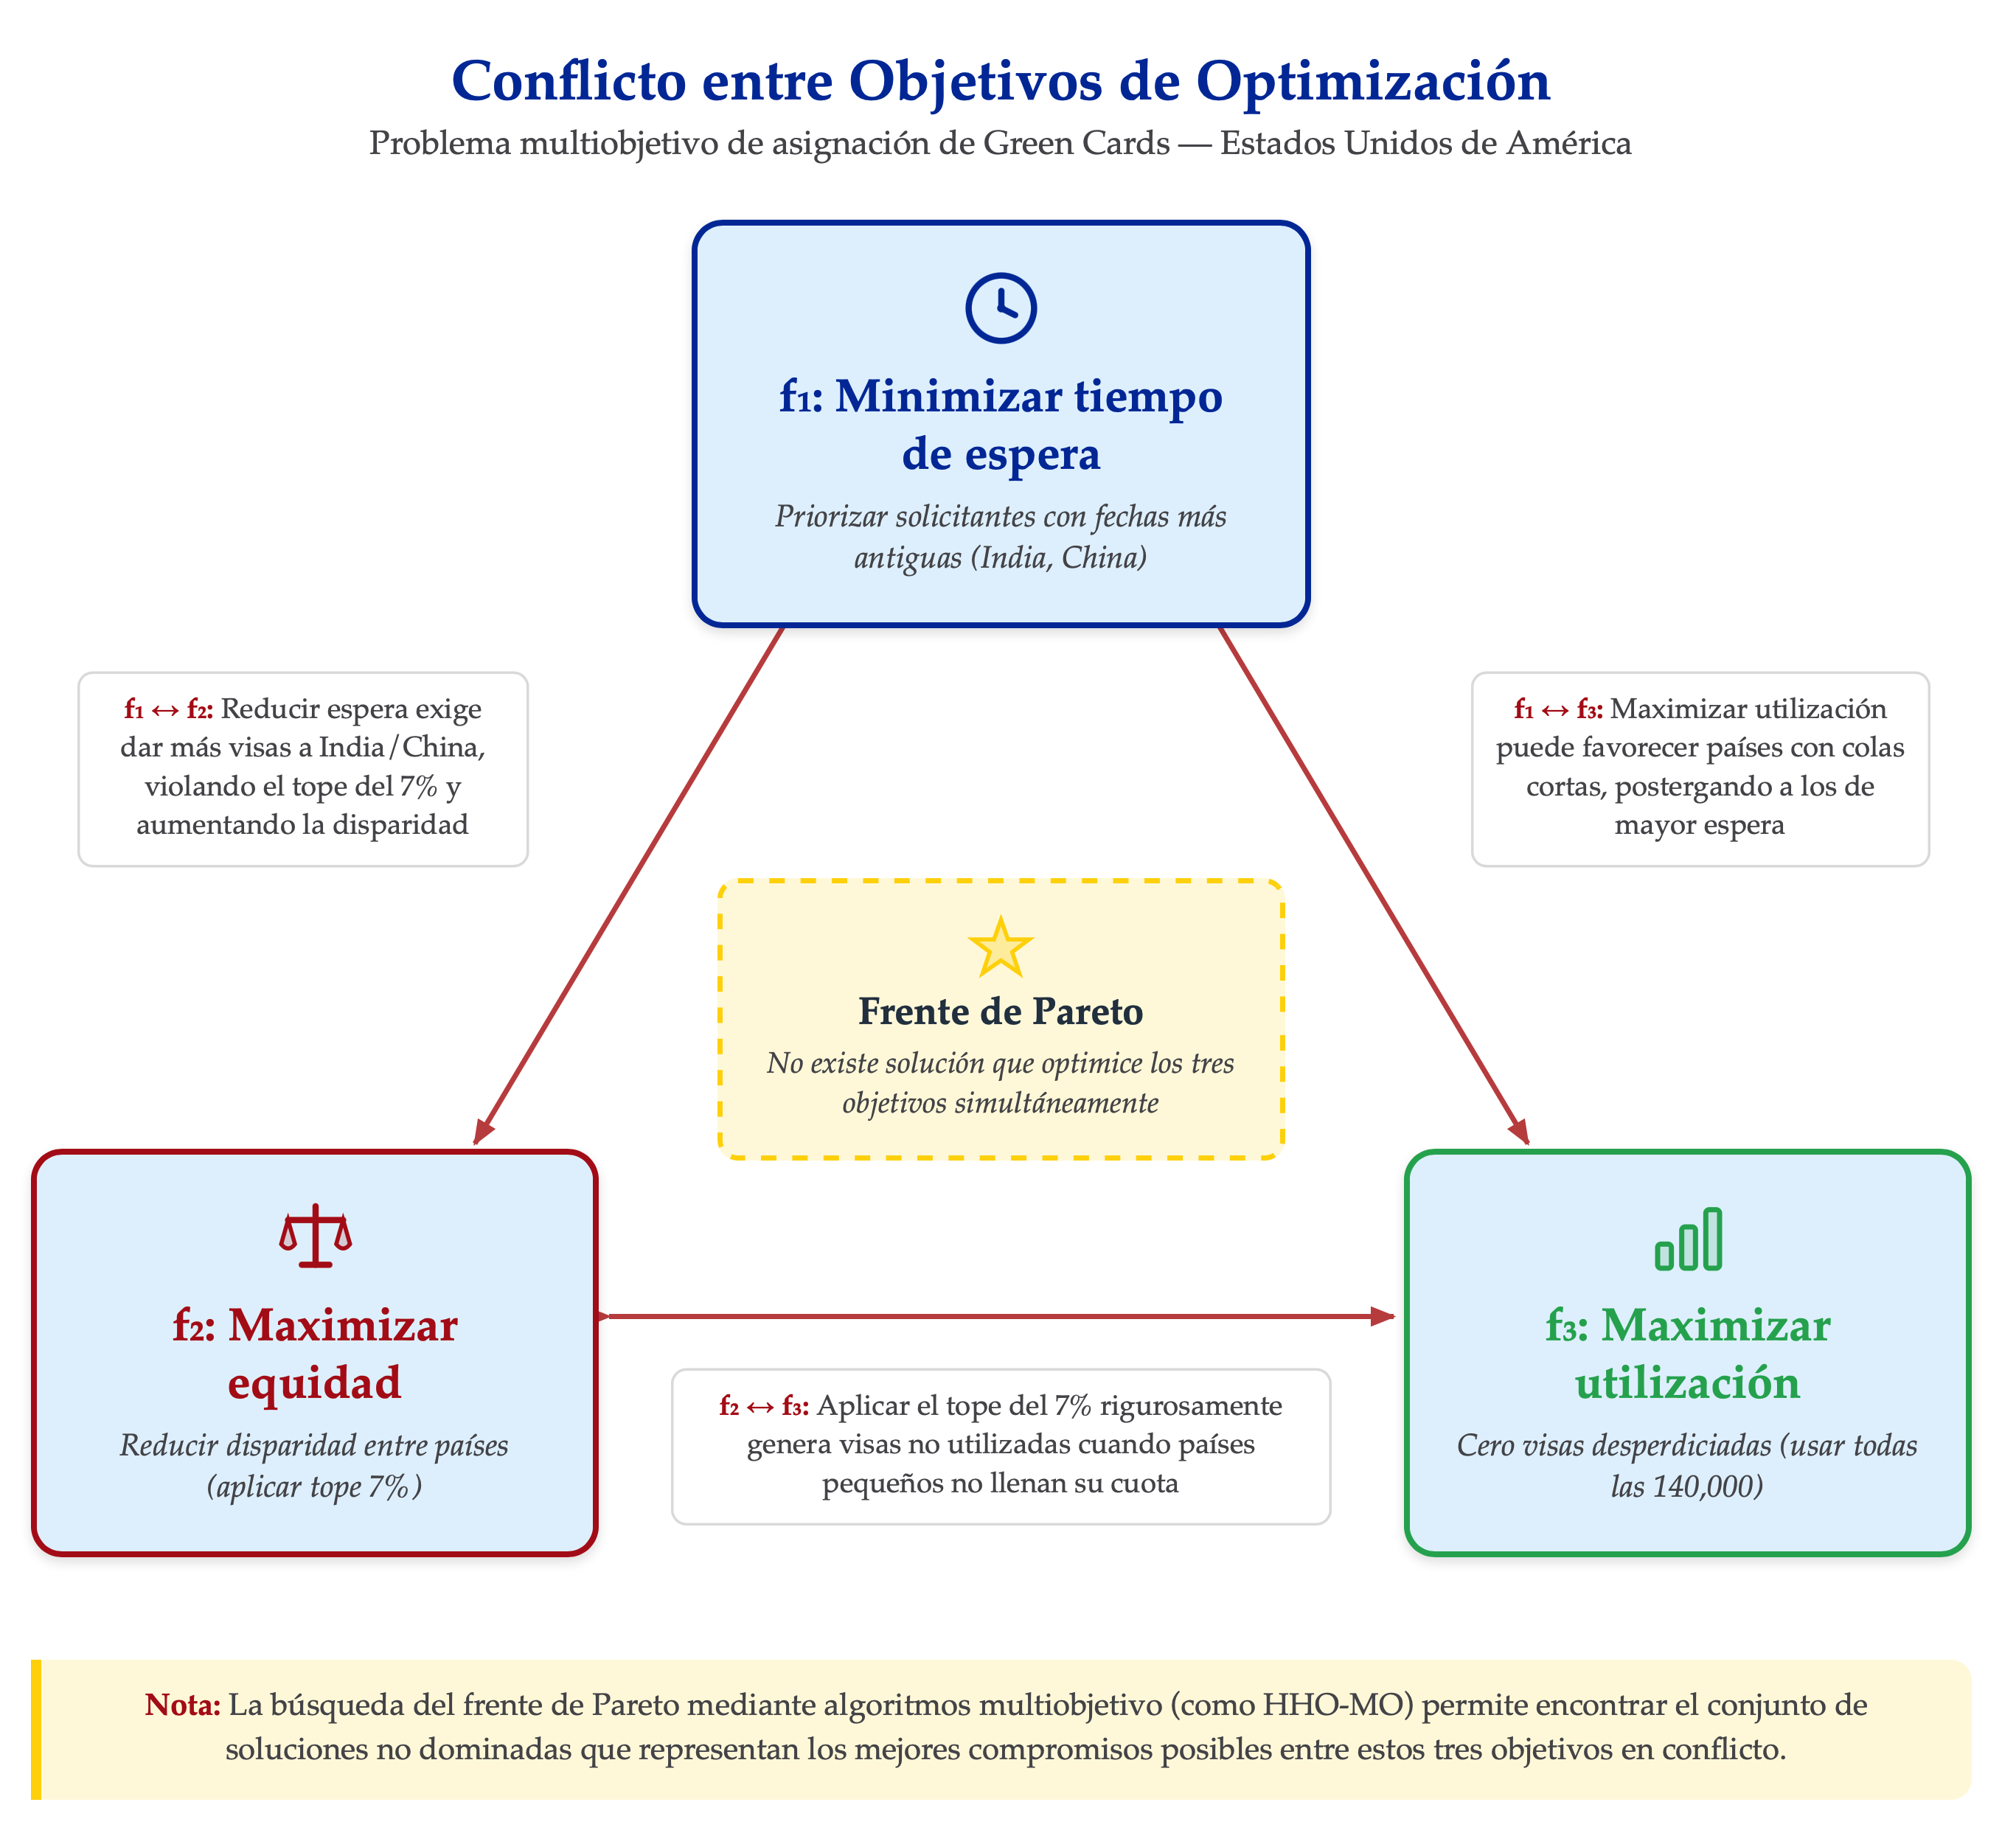
\includegraphics[width=0.80\textwidth]{conflicto_objetivos.png}
    \caption{Los tres objetivos en conflicto. Reducir la espera ($f_1$) exige concentrar visas en India/China, lo que dispara la disparidad ($f_2$); maximizar la equidad o la utilización desplaza a los grupos de mayor espera. No existe un único óptimo: existe un \emph{frente de Pareto}.}
    \label{fig:conflicto}
\end{figure}

\subsection{Formulación compacta y restricciones}
\begin{formulabox}
\begin{align*}
\min_{\mathbf{x}} \quad & \bigl\{ f_1(\mathbf{x}),\; f_2(\mathbf{x}),\; f_3(\mathbf{x}) \bigr\}\\[3pt]
\text{s.a.}\quad
& \text{R1: } \textstyle\sum_{g} x_g \leq V = 140{,}000 && \text{(visas totales)}\\
& \text{R2: } \textstyle\sum_{g:\,c(g)=c} x_g \leq P_c = 25{,}620 \;\; \forall c && \text{(tope del 7\,\% por país)}\\
& \text{R3: } \textstyle\sum_{g:\,j(g)=j} x_g \leq K_j^{\text{eff}} \;\; \forall j && \text{(tope efectivo por categoría)}\\
& \text{R4: } 0 \leq x_g \leq n_g \;\; \forall g && \text{(no exceder la demanda)}\\
& \text{R5: } x_g \in \mathbb{Z}^{+}_0 \;\; \forall g && \text{(enteros)}\\
& \text{R6: orden FIFO por par } (c,j) && \text{(antigüedad dentro de cada cola)}
\end{align*}
\end{formulabox}

Se trata de un problema de optimización combinatoria triobjetivo con seis restricciones, perteneciente a la clase \textbf{NP-Difícil} \parencite{gareyjohnson1979}: el espacio de asignaciones factibles crece de forma exponencial con $G$, lo que justifica el uso de una metaheurística en lugar de métodos exactos.

\subsection{Conceptos de optimalidad multiobjetivo}
\begin{formulabox}
\textbf{Dominancia de Pareto.} $\mathbf{x}$ domina a $\mathbf{x}'$ ($\mathbf{x} \prec \mathbf{x}'$) si y solo si
\(\forall i:\, f_i(\mathbf{x}) \leq f_i(\mathbf{x}') \;\wedge\; \exists i:\, f_i(\mathbf{x}) < f_i(\mathbf{x}').\)\\[3pt]
\textbf{Frente de Pareto.} $\mathcal{P}^* = \{\mathbf{x}\in\mathcal{F} \mid \nexists\, \mathbf{x}'\in\mathcal{F}:\mathbf{x}'\prec\mathbf{x}\}$, el conjunto de soluciones factibles no dominadas. El objetivo de MOHHO es \emph{aproximar} $\mathcal{P}^*$ mediante un archivo externo.
\end{formulabox}

% ==========================================================
\section{La metaheurística: MOHHO}
\label{sec:mohho}

\subsection{Fundamentos y por qué HHO}
Harris Hawks Optimization \parencite{heidari2019} es una metaheurística poblacional inspirada en la \textbf{caza cooperativa} de los halcones de Harris: varios halcones rodean a una presa (el conejo) y alternan rastreo, asedio y ataques sorpresa. No se abordó en el curso y posee una característica distintiva: una \textbf{transición continua entre exploración y explotación} gobernada por una sola variable física, la \emph{energía de escape} de la presa,
\[
E = 2E_0\Bigl(1 - \tfrac{t}{T}\Bigr), \qquad E_0 \sim U(-1,\,1),
\]
que decae con la iteración $t$. Cuando $|E|\geq 1$ la presa tiene energía para huir y los halcones \textbf{exploran} el espacio; cuando $|E|<1$ la presa se agota y los halcones \textbf{explotan} cerrando el cerco mediante asedios suaves o duros, con o sin inmersiones rápidas (saltos de Lévy).

\subsection{Operadores}
La adaptación multiobjetivo (MOHHO) sigue a \textcite{kusoglu2020} y \textcite{cerci2022}. Los \textbf{seis operadores} de movimiento se seleccionan según $|E|$ y $r$:

\begin{table}[H]
\centering
\renewcommand{\arraystretch}{1.25}
\small
\begin{tabular}{clp{8.6cm}}
\toprule
\rowcolor{tablehead}
\textcolor{white}{\textbf{Op.}} & \textcolor{white}{\textbf{Condición}} & \textcolor{white}{\textbf{Comportamiento}}\\
\midrule
OP1 & $|E|\geq1,\; q\geq0.5$ & Exploración desde un halcón aleatorio del enjambre.\\
\rowcolor{gray!8}
OP2 & $|E|\geq1,\; q<0.5$ & Exploración respecto al centro de masa de la población.\\
OP3 & $|E|\geq0.5,\; r\geq0.5$ & Asedio suave: acercamiento gradual a la presa.\\
\rowcolor{gray!8}
OP4 & $|E|<0.5,\; r\geq0.5$ & Asedio duro: contracción agresiva del cerco.\\
OP5 & $|E|\geq0.5,\; r<0.5$ & Asedio suave con inmersiones rápidas (salto de \textbf{Lévy}).\\
\rowcolor{gray!8}
OP6 & $|E|<0.5,\; r<0.5$ & Asedio duro con inmersiones rápidas (salto de \textbf{Lévy}).\\
\bottomrule
\end{tabular}
\caption{Los seis operadores de MOHHO. La memoria del algoritmo es el \emph{archivo externo} de no dominados; la presa (líder) se extrae de él.}
\end{table}

\begin{yellowbox}
\textbf{Adaptaciones multiobjetivo clave.} (1) \emph{Selección del líder}: la presa no es un único óptimo global, sino una solución elegida del archivo externo con probabilidad inversa a su \textit{crowding distance}, lo que favorece la diversidad. (2) \emph{Archivo externo} de hasta 100 soluciones no dominadas, podado por \textit{crowding distance} cuando se satura. (3) \emph{Actualización de no dominancia} tras cada iteración.
\end{yellowbox}

El Listado~\ref{lst:energia} muestra el núcleo de la implementación: la energía de escape y la ramificación de fase que selecciona el operador en cada iteración (extracto real de \texttt{core/hho.py} y \texttt{core/mohho.py}).

\begin{lstlisting}[style=vp,caption={Energía de escape y selección de fase (exploración / asedio / Lévy).},label={lst:energia}]
def escape_energy(t, max_t, rng):
    e0 = 2 * rng.random() - 1          # E0 ~ U(-1, 1)
    return 2 * e0 * (1 - t / max_t)    # |E| decae de 2 -> 0

# para cada halcon i, en cada iteracion t:
e = escape_energy(t, max_iter, rng); abs_e = abs(e)
rabbit = select_leader(archive, rng)   # lider por crowding distance
if abs_e >= 1:                         # EXPLORACION  (OP1 / OP2)
    new = exploration_step(pop, i, rabbit, x_mean, rng)
elif rng.random() >= 0.5:              # ASEDIO  (OP3 si |E|>=0.5, OP4 si <0.5)
    new = siege_step(pop[i], rabbit, e, abs_e, rng)
else:                                  # ASEDIO con salto de Levy (OP5 / OP6)
    new = levy_step(pop[i], rabbit, x_mean, e, abs_e, rng)
update_archive(archive, new, ...)      # inserta si no-dominado + poda
\end{lstlisting}

\subsection{Codificación SPV y decodificador de factibilidad garantizada}
Los operadores de HHO operan en el continuo $\mathbb{R}^{105}$, pero el problema es combinatorio. Se usa la regla \textbf{SPV} (\textit{Smallest Position Value}) de \textcite{bean1994}: cada halcón $\mathbf{H}\in\mathbb{R}^{105}$ se convierte en una \emph{permutación} $\boldsymbol{\pi}$ ordenando los índices por valor ascendente de $h_g$. Un \textbf{decodificador greedy} recorre los grupos en ese orden y asigna
\[
x_g = \min\!\bigl(n_g,\; V_{\text{res}},\; P_{c(g)}^{\text{res}},\; K_{j(g)}^{\text{res}}\bigr),
\]
decrementando los residuos de R1--R3 tras cada paso. Así, \textbf{toda} solución decodificada satisface R1--R6 por construcción, sin funciones de penalización ni operadores de reparación (Listado~\ref{lst:decoder}, extracto de \texttt{core/decoder.py}).

\begin{lstlisting}[style=vp,caption={Decodificador greedy: factibilidad garantizada por construcción.},label={lst:decoder}]
def decode(perm, groups, V, country_caps, category_caps):
    x = {g["index"]: 0 for g in groups}
    v_rem = V                       # residuo de R1 (visas totales)
    used_c, used_j = {}, {}         # residuos de R2 (pais) y R3 (categoria)
    for g_idx in perm:              # recorre los grupos en el orden SPV
        g = lookup[g_idx]
        cap_c = country_caps[g["country"]]  - used_c.get(g["country"], 0)
        cap_j = category_caps[g["category"]] - used_j.get(g["category"], 0)
        x[g_idx] = min(g["n"], v_rem, cap_c, cap_j)   # asignacion factible maxima
        v_rem -= x[g_idx]
        used_c[g["country"]]  = used_c.get(g["country"], 0)  + x[g_idx]
        used_j[g["category"]] = used_j.get(g["category"], 0) + x[g_idx]
    return x                        # cumple R1-R6 sin reparacion
\end{lstlisting}

\begin{resultbox}
\textbf{Flujo del algoritmo (pseudocódigo).}
\begin{enumerate}\setlength{\itemsep}{1pt}
    \item Inicializar $N$ halcones aleatorios en $\mathbb{R}^{105}$; decodificar (SPV $\to$ greedy) y construir el archivo inicial.
    \item \textbf{Para} $t=1\dots T$: actualizar energía $E$; seleccionar líder del archivo; mover cada halcón con OP1--OP6 según $|E|$ y $r$; decodificar y evaluar $(f_1,f_2,f_3)$; actualizar el archivo de no dominados.
    \item Retornar el archivo final como aproximación al frente de Pareto $\mathcal{P}^*$.
\end{enumerate}
\end{resultbox}

\subsection{Evidencia de funcionamiento: el algoritmo en vivo}
La plataforma \textbf{renderiza cada iteración del algoritmo real} sobre el espacio objetivo. Los \textbf{halcones} (triángulos) son soluciones candidatas posicionadas por sus valores $(f_1,f_2)$; el \textbf{conejo} rosa es la solución líder extraída del archivo; la línea azul es el \textbf{frente de Pareto} y la \texttt{X} roja marca al FIFO. El panel inferior derecho reporta en todo momento la fase, la energía $E(t)$ y el tamaño del archivo. El color de los halcones codifica la fase activa: \textcolor{blue!70!black}{\textbf{azul}} = exploración, \textcolor{orange!80!black}{\textbf{amarillo}} = transición, \textcolor{red!70!black}{\textbf{naranja}} = asedio. La Figura~\ref{fig:canvas} muestra un instante de ese lienzo en plena fase de transición.

\begin{figure}[H]
    \centering
    \shot[0.86\textwidth]{sim_hawkhunt.png}
    \caption{Un instante del lienzo en vivo (fase de \textit{transición}, iteración 50/100). Cada triángulo es un halcón coloreado por su fase; el punto rosa es el conejo (solución líder extraída del archivo); la curva azul es el frente de Pareto y la \texttt{X} roja marca al FIFO. El panel inferior derecho reporta la fase, la energía $E(t)=1.00$ y el tamaño del archivo (94 soluciones). Las flechas amarillas son los saltos de L\'evy que escapan de óptimos locales.}
    \label{fig:canvas}
\end{figure}

La secuencia de la Figura~\ref{fig:hunt} captura \textbf{el flujo completo de la cacería} a lo largo de una corrida (40 halcones, 220 iteraciones), evidenciando que la transición exploración$\to$explotación gobernada por la energía $E=2E_0(1-t/T)$ se ejecuta exactamente como predice el diseño teórico de HHO.

\newcommand{\huntshot}[2]{\begin{minipage}[t]{0.485\textwidth}\centering\shot[\dimexpr\linewidth-2\fboxrule\relax]{#1}\\[2pt]{\footnotesize\color{headerblue}#2}\end{minipage}}

\begin{figure}[htbp]
\centering
\huntshot{hunt_1_exploracion.png}{\textbf{1. Exploración} ($E\!\approx\!1.9$): halcones dispersos, búsqueda global (OP1/OP2)}\hfill
\huntshot{hunt_2_exploracion2.png}{\textbf{2. Exploración} ($E\!\approx\!1.6$): el frente de Pareto empieza a formarse}\\[8pt]
\huntshot{hunt_3_transicion.png}{\textbf{3. Transición} ($E\!\approx\!1.2$): saltos de L\'evy escapan óptimos locales (OP3/OP5)}\hfill
\huntshot{hunt_4_transicion2.png}{\textbf{4. Transición} ($E\!\approx\!0.7$): el frente se define y ya domina al FIFO}\\[8pt]
\huntshot{hunt_5_asedio.png}{\textbf{5. Asedio} ($E\!\approx\!0.3$): cerco cooperativo en anillos (OP4/OP6)}\hfill
\huntshot{hunt_6_captura.png}{\textbf{6. Captura} ($E\!\to\!0$): frente convergido; los halcones atrapan al conejo}
\caption{Flujo completo de la cacería MOHHO en vivo: de la exploración dispersa ($E$ alta) al asedio cooperativo y la captura ($E\!\to\!0$). El cambio de color (azul$\to$amarillo$\to$naranja$\to$verde) refleja el decaimiento de la energía de escape iteración a iteración.}
\label{fig:hunt}
\end{figure}

% ==========================================================
\section{Plataforma de implementación: Visa Predict AI}
\label{sec:plataforma}

La implementación se realizó en \textbf{Python 3.12} (núcleo del algoritmo y API) y \textbf{Nuxt~4 / TypeScript} (interfaz). La arquitectura desacopla cuatro capas (Figura~\ref{fig:arch}): interfaz, API REST\,+\,WebSocket, núcleo de optimización y datos. El núcleo es agnóstico a la interfaz: el mismo optimizador alimenta tanto las corridas en lote (reproducibles) como el \textit{streaming} en vivo vía WebSocket.

\begin{figure}[htbp]
    \centering
    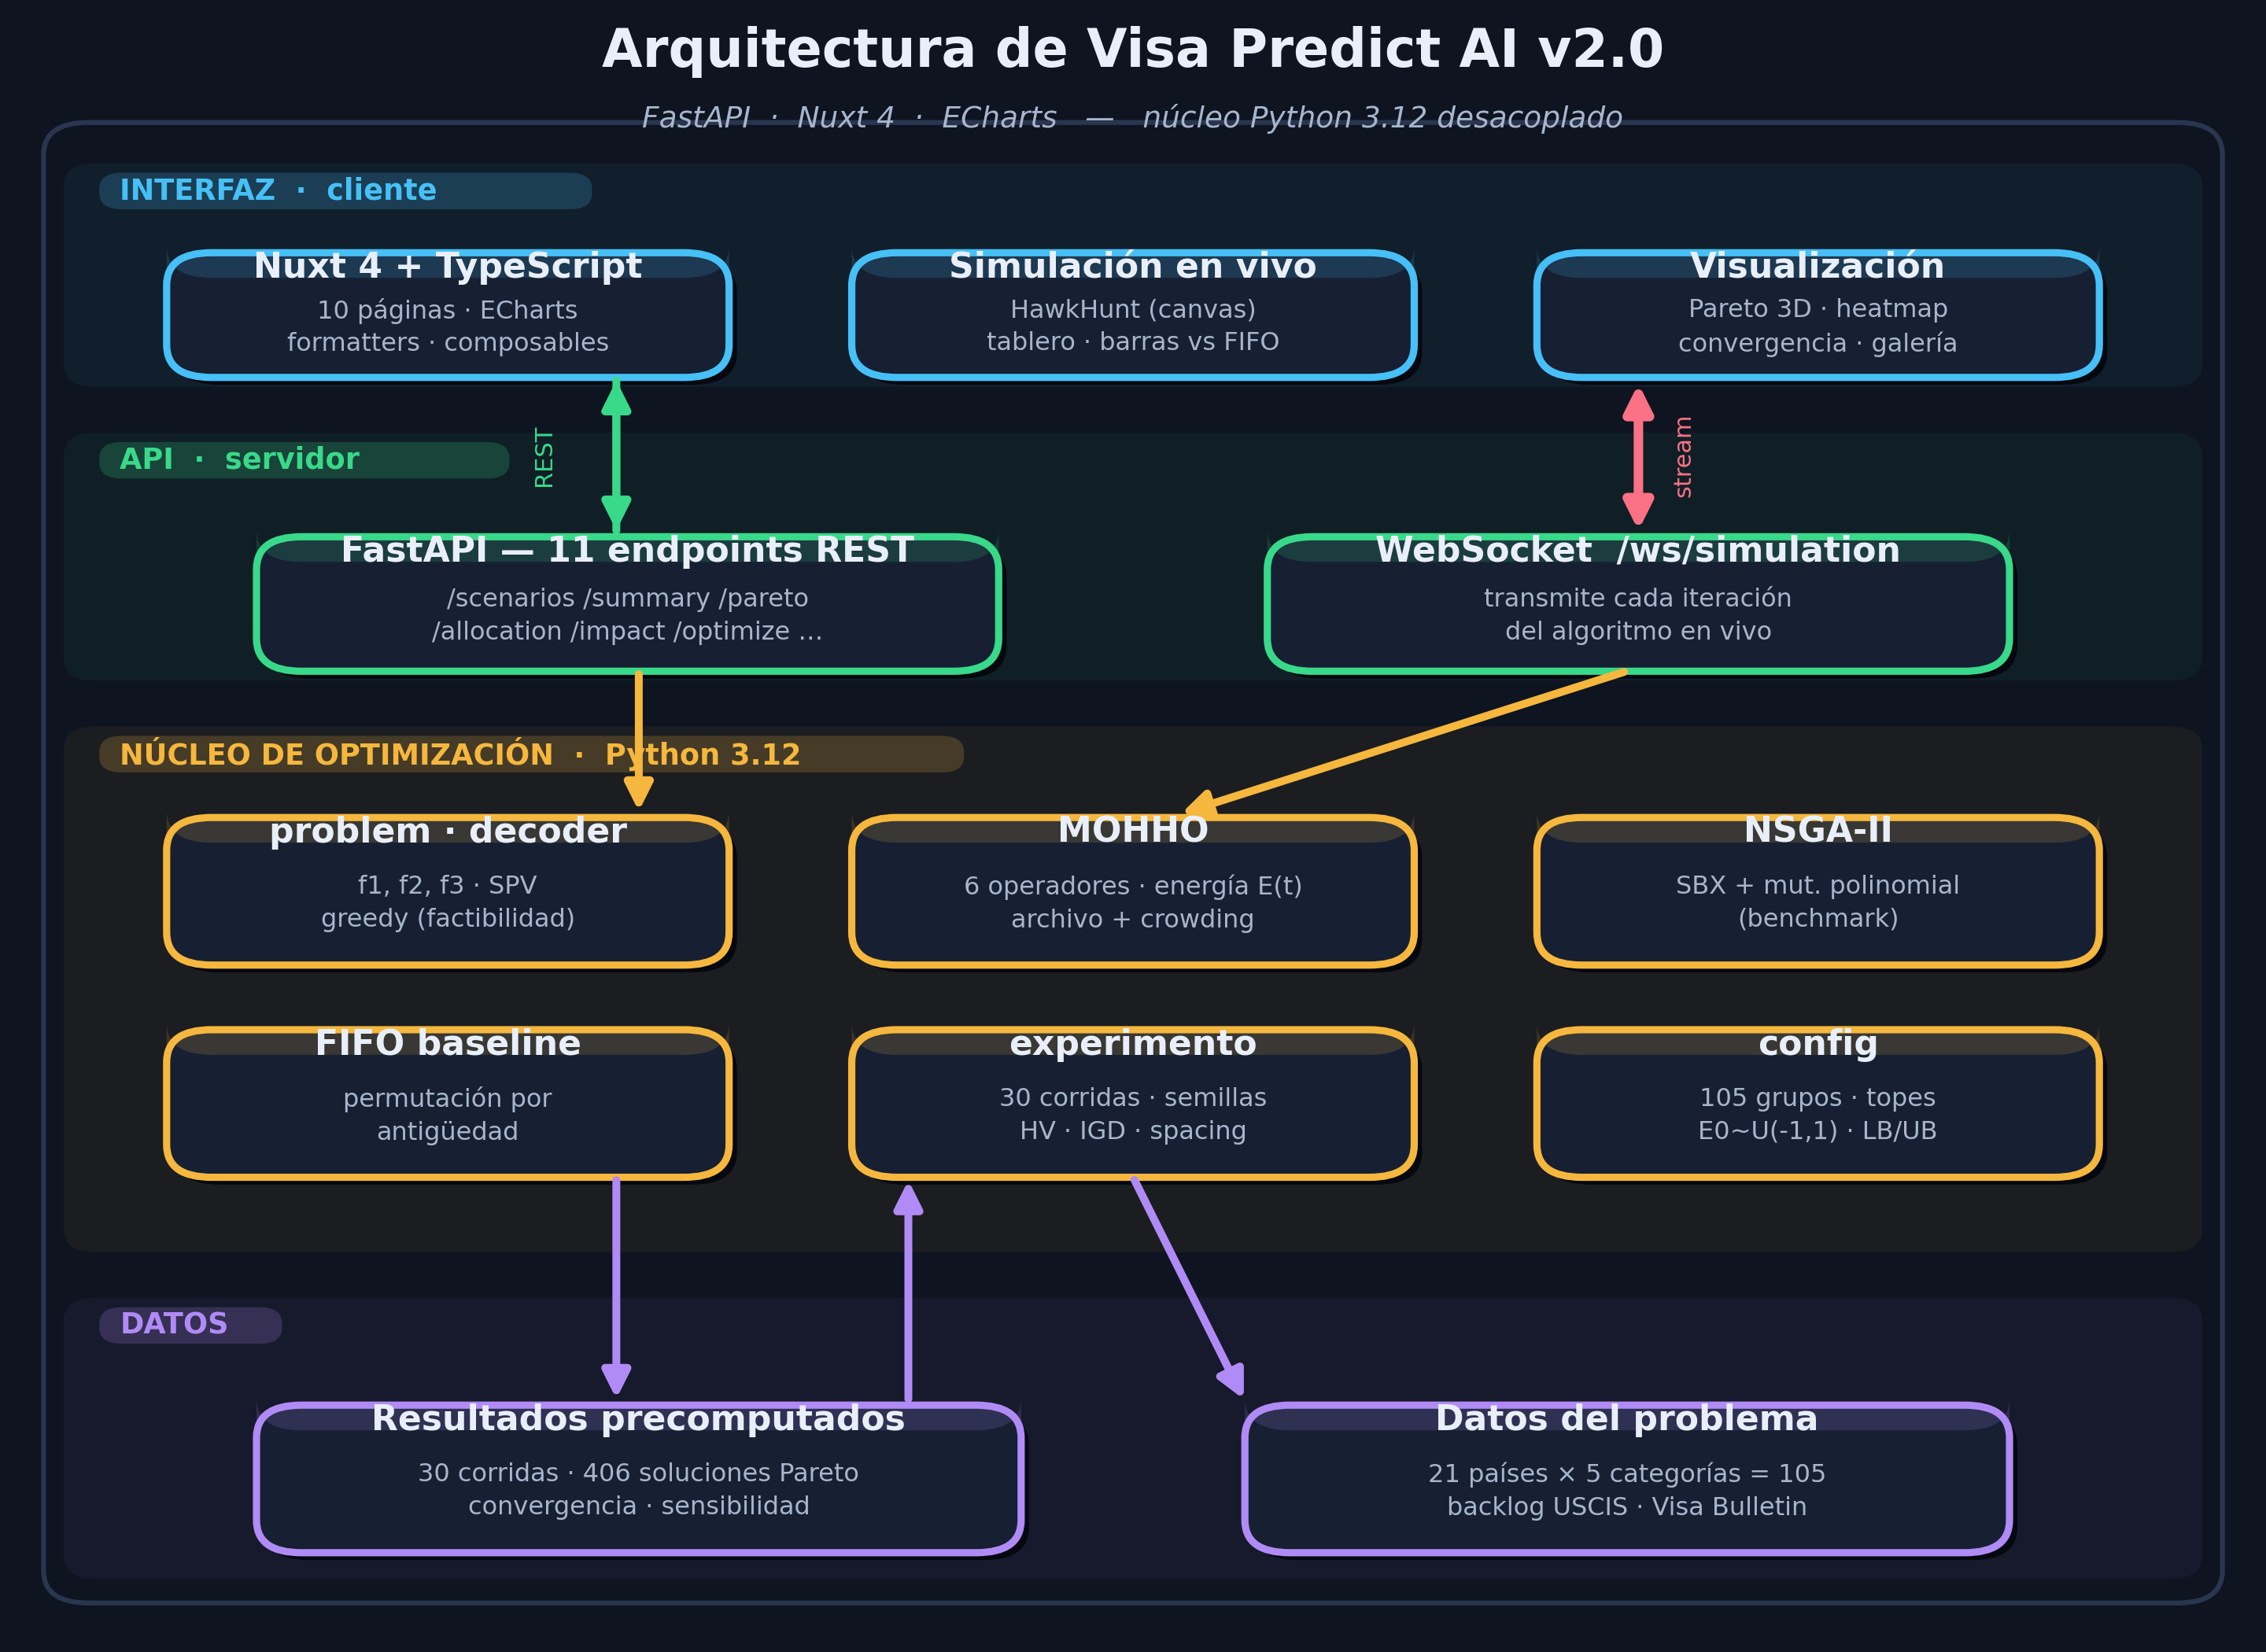
\includegraphics[width=0.97\textwidth]{architecture.png}
    \caption{Arquitectura desacoplada de \textbf{Visa Predict AI v2.0}. La interfaz consume la API por REST y recibe cada iteración del algoritmo por WebSocket; el núcleo Python alberga el problema, el decodificador, MOHHO, NSGA-II y la línea base FIFO sobre los mismos datos.}
    \label{fig:arch}
\end{figure}

\begin{table}[H]
\centering
\renewcommand{\arraystretch}{1.3}
\small
\begin{tabular}{lp{10.2cm}}
\toprule
\rowcolor{tablehead}
\textcolor{white}{\textbf{Capa / módulo}} & \textcolor{white}{\textbf{Responsabilidad}}\\
\midrule
\texttt{core/problem, decoder} & Datos del problema, funciones $f_1$--$f_3$ y decodificador greedy de factibilidad garantizada.\\
\rowcolor{gray!8}
\texttt{core/hho, mohho} & Operadores OP1--OP6, energía $E(t)$, archivo externo y poda por \textit{crowding distance}.\\
\texttt{core/fifo} & Línea base FIFO determinista (permutación por antigüedad).\\
\rowcolor{gray!8}
\texttt{api + ws/simulation} & 11 endpoints REST y un WebSocket (\texttt{/ws/simulation}) que transmite cada iteración en vivo.\\
\texttt{frontend (Nuxt+ECharts)} & 10 páginas: modelo, Pareto, asignación, impacto, convergencia y \textbf{simulación en tiempo real}.\\
\bottomrule
\end{tabular}
\caption{Arquitectura de \textbf{Visa Predict AI v2.0}. El optimizador puede ejecutarse en lote (resultados reproducibles) o en streaming vía WebSocket para la visualización en vivo.}
\end{table}

El \textbf{tablero de control} de la simulación (Figura~\ref{fig:dashboard}) expone el estado interno del algoritmo en tiempo real: el medidor de energía $E(t)$ y la fase activa, el contador de iteraciones, el número de soluciones en el archivo, el hipervolumen acumulado y su velocidad de crecimiento $\Delta\text{HV/iter}$. Las barras de la Figura~\ref{fig:racebars} comparan, iteración a iteración, el mejor valor de cada objetivo contra la referencia FIFO (línea roja).

\begin{figure}[htbp]
    \centering
    \shot[0.97\textwidth]{sim_dashboard.png}
    \caption{Tablero de control de la simulación: energía $E(t)=1.06$ (fase de transición), iteración 47/100, 90 soluciones Pareto, hipervolumen $1{,}747{,}182$ y crecimiento $\Delta\text{HV}=+8398$/iter.}
    \label{fig:dashboard}
\end{figure}

\begin{figure}[htbp]
    \centering
    \shot[0.97\textwidth]{sim_racebars.png}
    \caption{Objetivos en tiempo real frente a la línea base FIFO. MOHHO mejora $f_2$ en un 80.5\,\% (de 12.64 a 2.46 años) y reduce $f_3$ casi a cero, manteniendo $f_1$ por debajo del FIFO.}
    \label{fig:racebars}
\end{figure}

\clearpage
\subsection{Recorrido por las diez secciones de la plataforma}
\label{sec:recorrido}
La aplicación organiza el proyecto en \textbf{diez secciones navegables}. Su pieza central es el frente de Pareto interactivo en 3D (Figura~\ref{fig:gal-3d}); a continuación se recorren las diez con capturas de la herramienta en ejecución, que evidencian el alcance del trabajo realizado: desde el planteamiento del modelo hasta la simulación del algoritmo en vivo y el análisis comparativo.

\begin{figure}[H]
    \centering
    \shot[0.92\textwidth]{app_pareto_3d.png}
    \caption{Pieza central de la plataforma: el \textbf{frente de Pareto interactivo en 3D} ($f_1$ carga de espera, $f_2$ disparidad, $f_3$ desperdicio). Cada punto es una de las 406 políticas no dominadas; el FIFO (punto rosa) flota dominado por encima del frente. El usuario rota la vista, hace \textit{zoom} y alterna con las tres proyecciones 2D.}
    \label{fig:gal-3d}
\end{figure}

\newcommand{\galbig}[2]{\begin{minipage}[t]{0.485\textwidth}\centering\shot[\dimexpr\linewidth-2\fboxrule\relax]{#1}\\[3pt]{\footnotesize\color{headerblue}#2}\end{minipage}}

\noindent\galbig{gallery_index.png}{\textbf{1. Inicio}: visión general del proyecto y métricas clave}\hfill
\galbig{gallery_modelo.png}{\textbf{2. Modelo}: las tres funciones objetivo y las restricciones}\par\vspace{12pt}

\noindent\galbig{gallery_algoritmo.png}{\textbf{3. Algoritmo}: MOHHO, los seis operadores y la energía de escape}\hfill
\galbig{gallery_pareto.png}{\textbf{4. Pareto}: frente no dominado interactivo en 2D y 3D}\par\vspace{12pt}

\noindent\galbig{gallery_asignacion.png}{\textbf{5. Asignación}: visas recomendadas por país y categoría}\hfill
\galbig{gallery_impacto.png}{\textbf{6. Impacto}: diferencia de cada país frente al FIFO}\par\vspace{12pt}

\noindent\galbig{gallery_convergencia.png}{\textbf{7. Convergencia}: evolución del hipervolumen en 30 corridas}\hfill
\galbig{gallery_simulacion.png}{\textbf{8. Simulación}: MOHHO ejecutándose en vivo, iteración a iteración}\par\vspace{12pt}

\noindent\galbig{gallery_datos.png}{\textbf{9. Datos}: demanda (\textit{backlog}) por grupo país$\times$categoría}\hfill
\galbig{gallery_analisis.png}{\textbf{10. Análisis}: métricas, comparación con NSGA-II y sensibilidad}\par\vspace{6pt}

% ==========================================================
\section{Diseño experimental y configuración}
\label{sec:experimental}

\subsection{Parámetros y criterio de parada}
Los resultados reportados provienen de un experimento en lote de \textbf{30 corridas independientes} (semillas 42--71) con la configuración de la Tabla~\ref{tab:params}. El modo interactivo de la web usa una configuración más ligera (30 halcones, 100 iteraciones) para mantener la fluidez visual; ambos comparten el mismo núcleo algorítmico.

\begin{table}[H]
\centering
\renewcommand{\arraystretch}{1.05}
\footnotesize\linespread{1.0}\selectfont
\begin{tabular}{l l >{\raggedright\arraybackslash}p{6.1cm}}
\toprule
\rowcolor{tablehead}
\textcolor{white}{\textbf{Parámetro}} & \textcolor{white}{\textbf{Valor}} & \textcolor{white}{\textbf{Justificación / nota}}\\
\midrule
\multicolumn{3}{l}{\cellcolor{headerblue!14}\textbf{Problema}}\\
Visas totales $V$ & 140{,}000 & Cupo anual EB del Congreso \parencite{crs2023}.\\
Países $C$ / categorías & 21 / 5 & 20 países nombrados $+$ \textit{Resto del Mundo}; $\times\,5$ EB $\Rightarrow G=105$.\\
Tope por país $P_c$ & 25{,}620 & 7\,\% de 366{,}000 (regla legal).\\
Demanda total $\sum n_g$ & 868{,}098 & Backlog USCIS / \textit{Visa Bulletin} \parencite{dosfeb2026,uscis2023}.\\
Variable $x_g$ & $\mathbb{Z}^{+}_0$, dim.\ 105 & Visas por grupo país$\times$categoría.\\
Cotas SPV $[LB,UB]$ & $[0,\,1]$ & Espacio continuo decodificado por SPV.\\
\midrule
\multicolumn{3}{l}{\cellcolor{sectiongreen!16}\textbf{Comunes a MOHHO y NSGA-II}}\\
Población $N$ & 50 & Estándar en metaheurísticas poblacionales.\\
Iteraciones / gen.\ $T$ & 500 & Converge antes de iter 150; margen amplio (§\ref{sec:critico}).\\
Corridas independientes & 30 & Significancia estadística de resultados estocásticos.\\
Codificación & SPV $+$ greedy & Factibilidad garantizada; \emph{idéntica} en ambos.\\
\midrule
\multicolumn{3}{l}{\cellcolor{exampleborder!22}\textbf{MOHHO}}\\
Energía de escape & $E=2E_0(1-t/T),\ E_0\!\sim\!U(-1,\,1)$ & Transición exploración/explotación \parencite{heidari2019}.\\
Operadores & OP1--OP6 & Seleccionados por $|E|$ y $r$ (§\ref{sec:mohho}).\\
Archivo externo & 100 & Validado: $\Delta$HV $<0.03\%$ vs.\ 500 (§\ref{sec:critico}).\\
Líder / poda & \textit{crowding distance} & Favorece la diversidad del frente.\\
Semillas & 42--71 & 30 corridas independientes.\\
\midrule
\multicolumn{3}{l}{\cellcolor{alertred!12}\textbf{NSGA-II (benchmark)}}\\
Cruce & SBX, $\eta_c=20$, $p_c=0.9$ & Configuración estándar \parencite{deb2002}.\\
Mutación & polinomial, $\eta_m=20$, $p_m=1/d$ & Estándar ($d=105$).\\
Selección / reemplazo & torneo binario / $(\mu+\lambda)$ elitista & Por rango y \textit{crowding}.\\
Semillas & 1--30 & 30 corridas independientes.\\
\midrule
\multicolumn{3}{l}{\cellcolor{headerblue!14}\textbf{Evaluación}}\\
Punto de referencia HV & $(10;\,16;\,50{,}000)$ & Cota superior de cada objetivo.\\
Criterio de parada & $T$ iteraciones fijas & Ganancia $<0.5\%$ tras la iteración 300.\\
Métricas & HV, IGD, \textit{spacing}, $|\mathcal{P}|$ & Convergencia, uniformidad y cardinalidad.\\
\bottomrule
\end{tabular}
\caption{Configuración experimental completa: problema, parámetros comunes, MOHHO, NSGA-II y evaluación.}
\label{tab:params}
\end{table}

\subsection{Datos de entrada}
Año fiscal 2026: $V=140{,}000$ visas; $C=21$ países (India, China, Filipinas, México, $\dots$, y \textit{Resto del Mundo}); 5 categorías EB; tope por país $P_c=25{,}620$ (7\,\% de 366{,}000) \parencite{crs2023}. La demanda $n_g$ se estima del backlog de peticiones I-140/I-360/I-526 (USCIS) y de las fechas de prioridad del \textit{Visa Bulletin} \parencite{dosfeb2026,uscis2023}.

\subsection{Métricas de evaluación}
\textbf{(1) Hipervolumen (HV)}: volumen del espacio objetivo 3D dominado por el frente respecto al punto de referencia $(10;\,16;\,50{,}000)$ (mayor es mejor, integra convergencia y diversidad). \textbf{(2) Cardinalidad} del frente no dominado. \textbf{(3) Frente combinado}: unión de los 30 frentes, refiltrada por no dominancia.

\subsection{Línea base: el sistema FIFO}
La permutación FIFO ordena los grupos por fecha de prioridad ascendente y se decodifica con el mismo greedy, produciendo una referencia determinista:

\begin{resultbox}
\textbf{FIFO:} $f_1 = 7.2138$,\quad $f_2 = 12.6377$ años,\quad $f_3 = 17{,}540$ visas desperdiciadas.\\
Logra una espera moderada porque prioriza la antigüedad, pero genera \textbf{alta disparidad} (concentra las visas en pocos países) y \textbf{desperdicia 17{,}540 visas} por el choque entre topes por país (R2) y por categoría (R3).
\end{resultbox}

% ==========================================================
\section{Resultados y desempeño}
\label{sec:resultados}

\subsection{Frente de Pareto combinado (406 soluciones)}
Tras combinar y refiltrar las 30 corridas, el frente contiene \textbf{406 soluciones no dominadas}. La Figura~\ref{fig:pareto3d} lo muestra en el espacio tridimensional completo $(f_1, f_2, f_3)$ y la Figura~\ref{fig:pareto} en su proyección $f_1$--$f_2$. Sus extremos revelan los compromisos del problema (Tabla~\ref{tab:extremos}).

\begin{figure}[htbp]
    \centering
    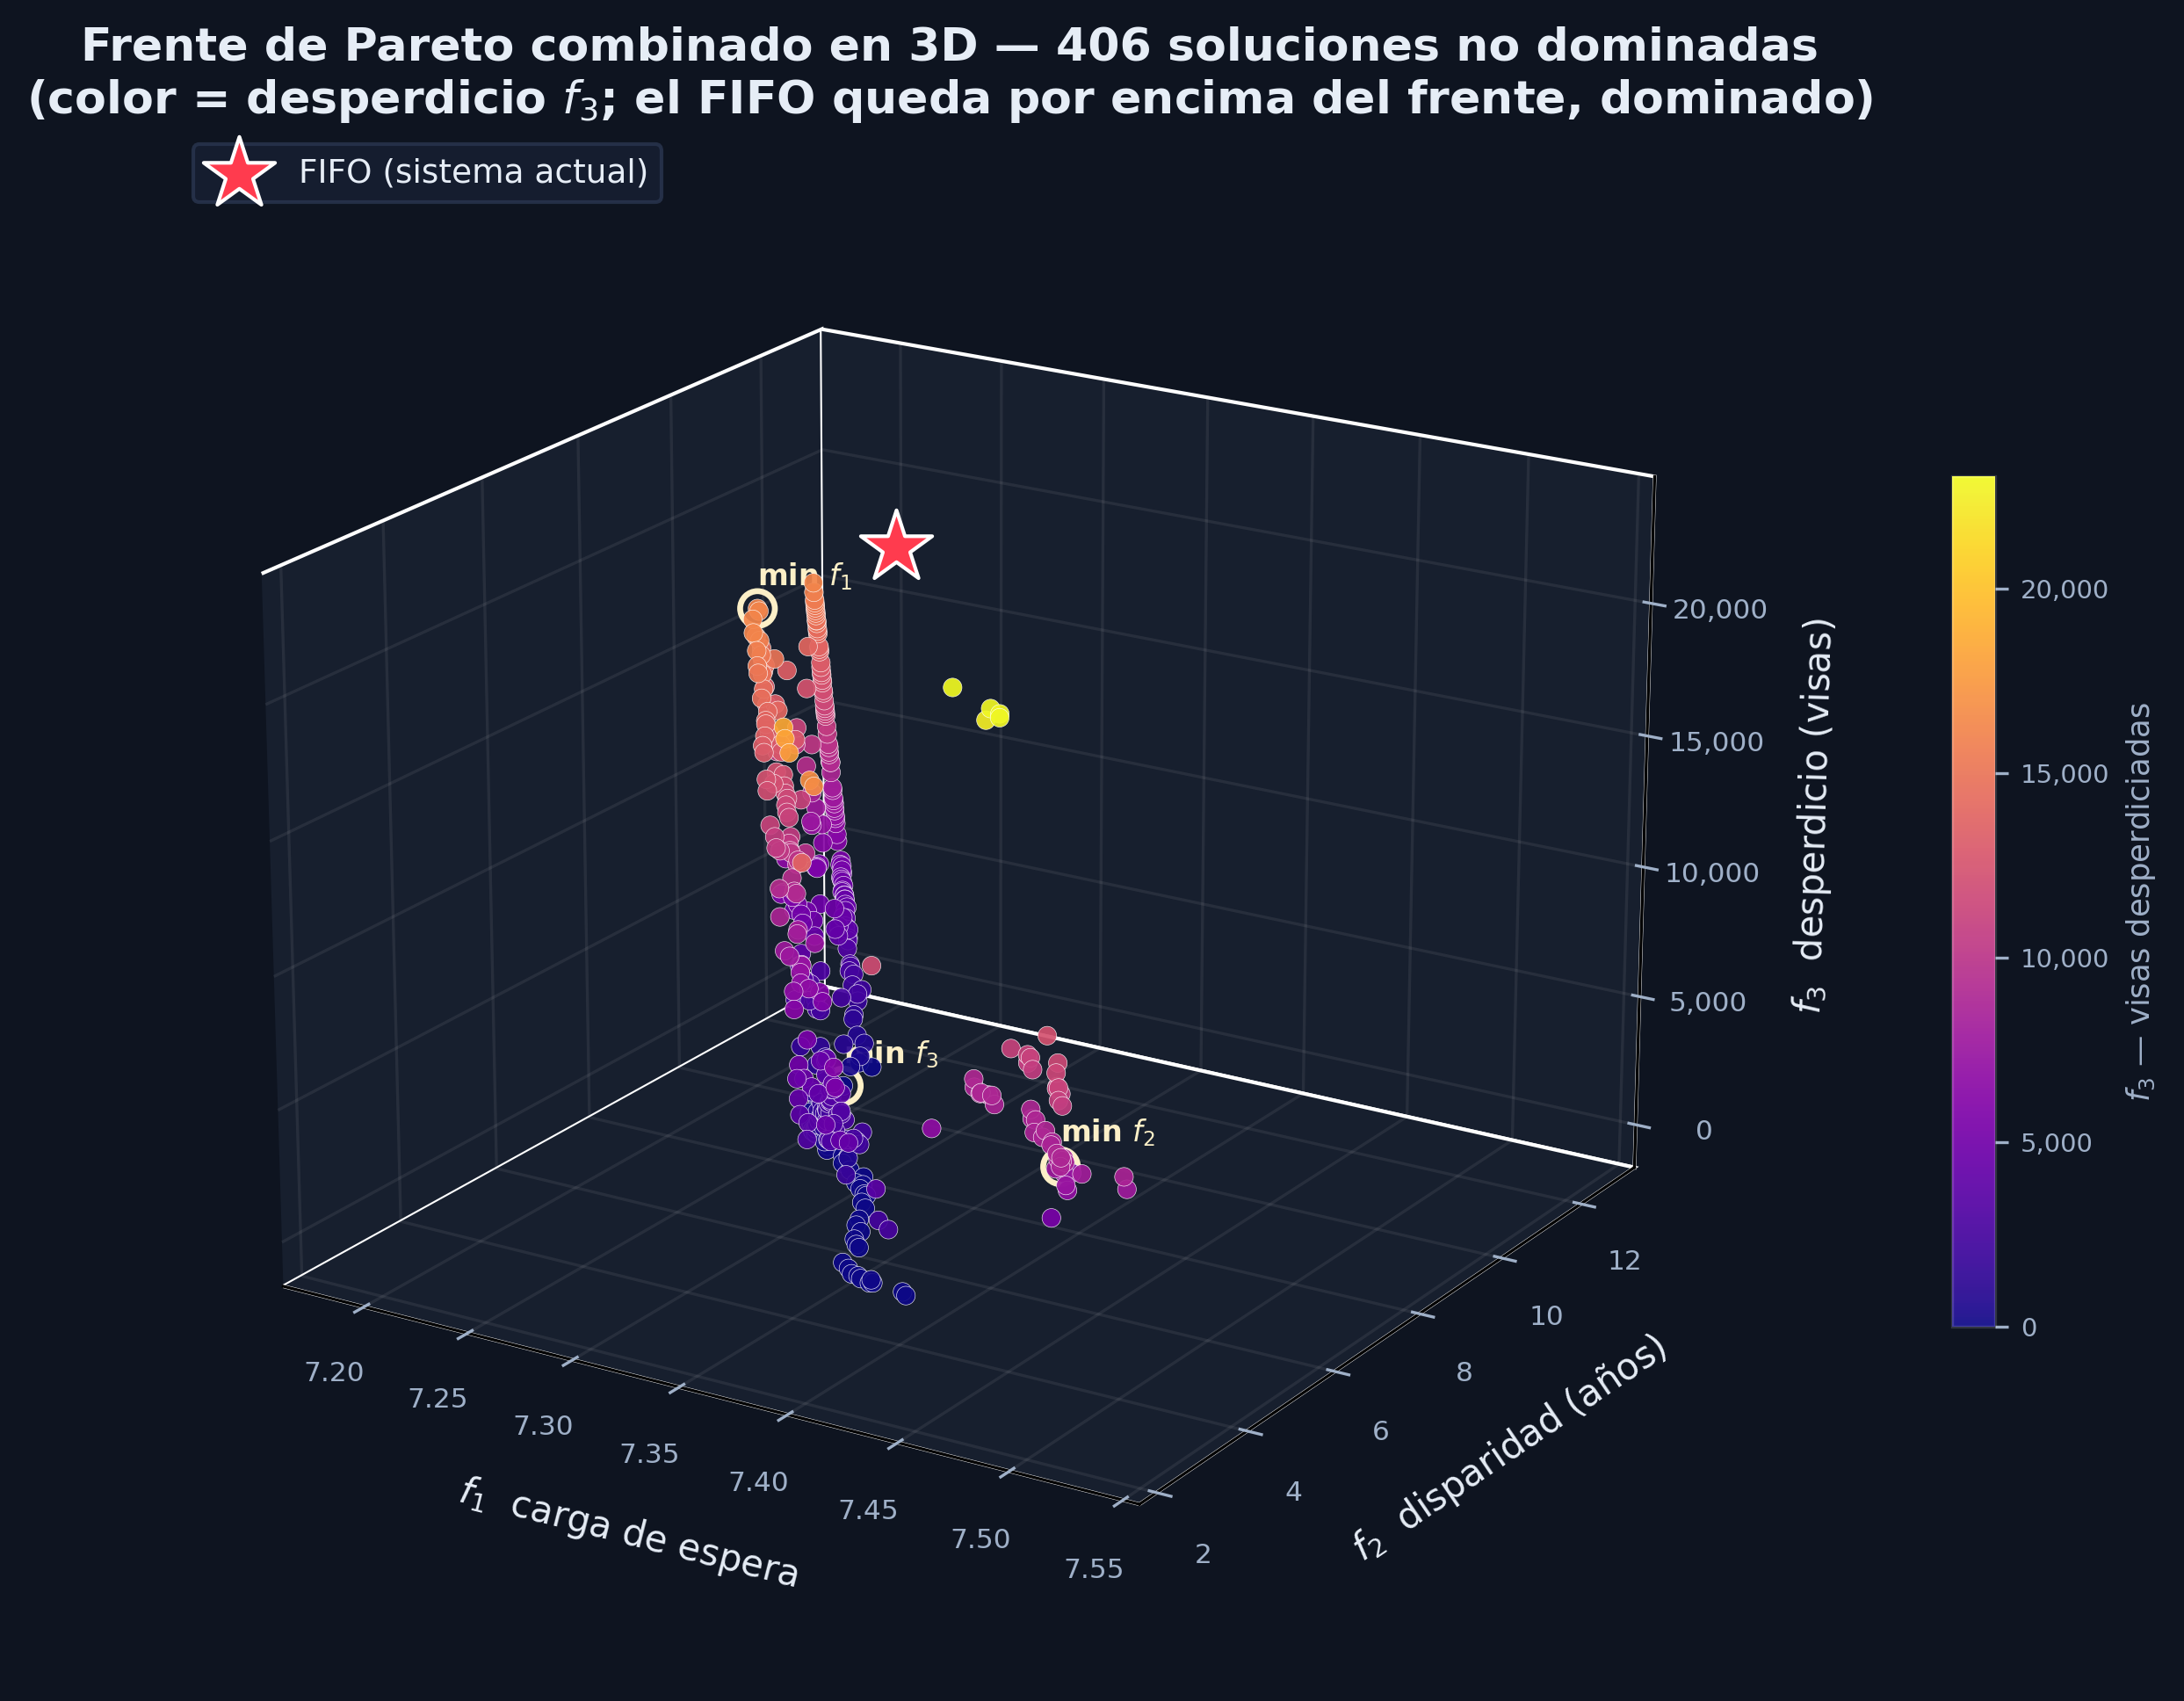
\includegraphics[width=0.97\textwidth]{fig_pareto3d.png}
    \caption{Frente de Pareto combinado en \textbf{3D}: las 406 soluciones no dominadas en el espacio de los tres objetivos, coloreadas por $f_3$ (desperdicio). El punto FIFO (estrella roja) flota \emph{por encima} del frente, evidencia visual de que es una solución dominada. Los círculos marcan las soluciones extremas (mínimo $f_1$, $f_2$ y $f_3$).}
    \label{fig:pareto3d}
\end{figure}

\begin{figure}[htbp]
    \centering
    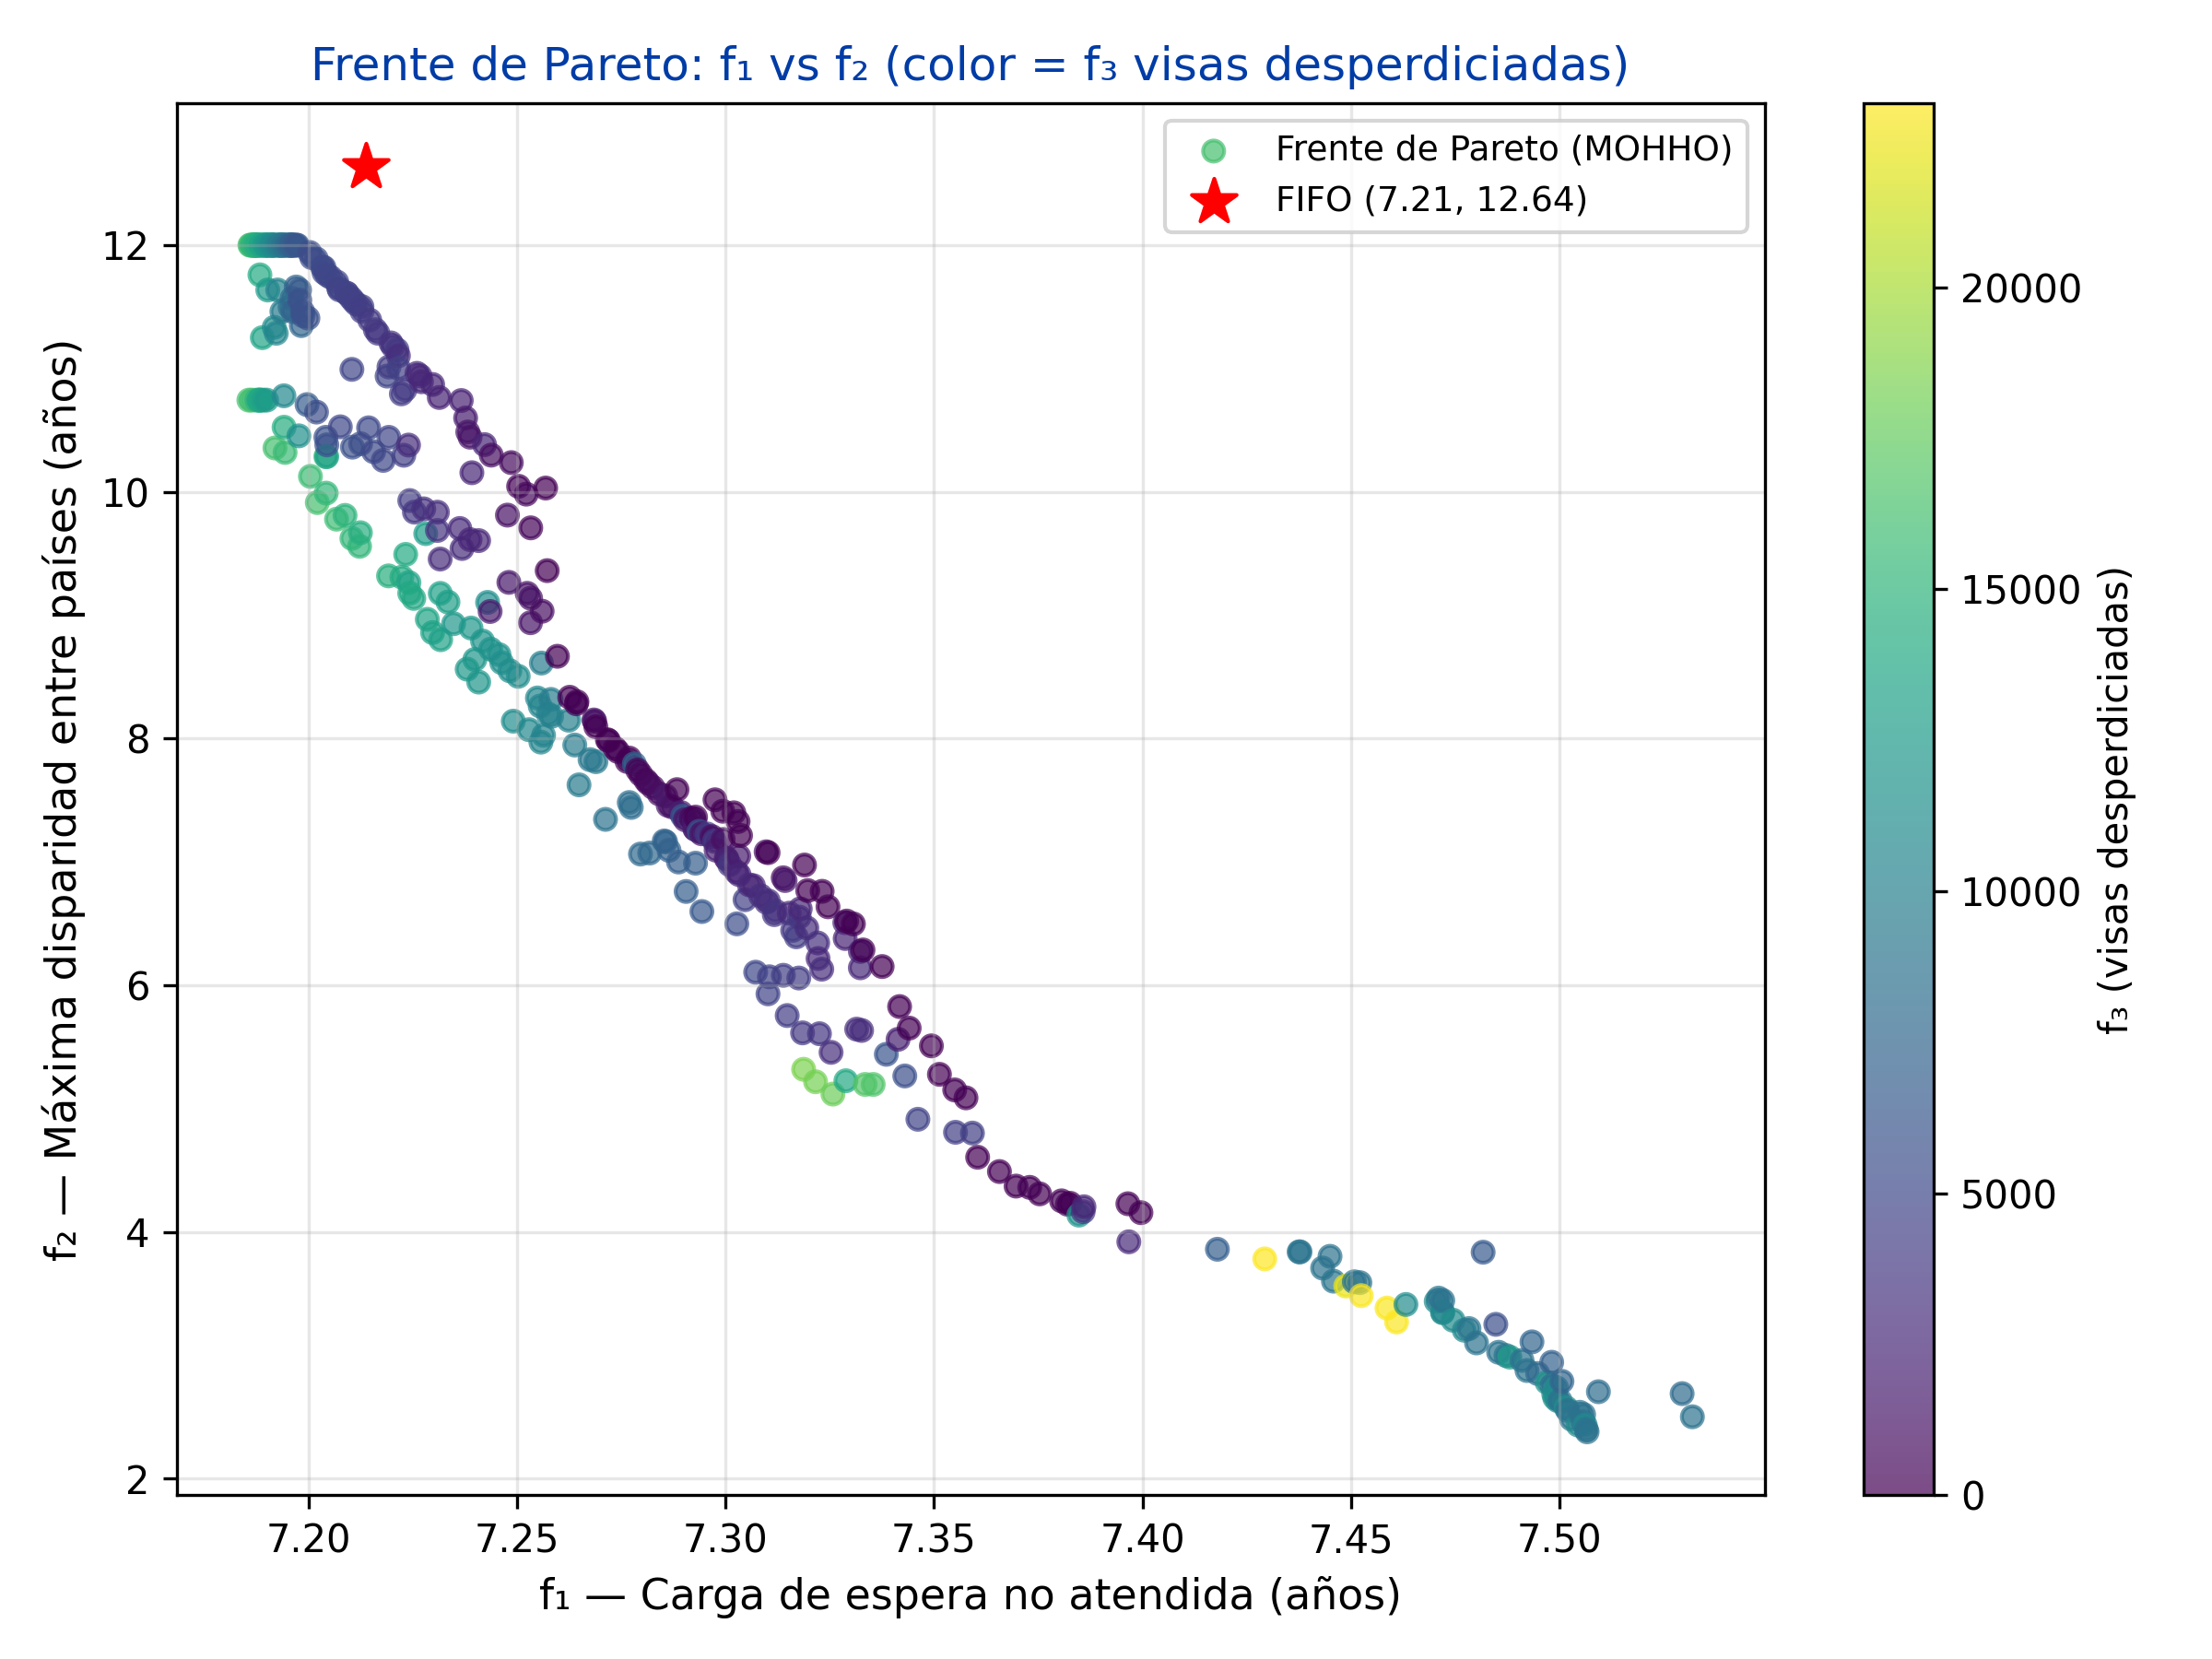
\includegraphics[width=0.82\textwidth]{pareto_front.png}
    \caption{Proyección $f_1$--$f_2$ del mismo frente combinado. El color codifica $f_3$ (desperdicio). El punto FIFO queda \emph{dentro} de la región dominada por el frente.}
    \label{fig:pareto}
\end{figure}

\begin{table}[H]
\centering
\renewcommand{\arraystretch}{1.3}
\small
\begin{tabular}{lcccl}
\toprule
\rowcolor{tablehead}
\textcolor{white}{\textbf{Solución}} & \textcolor{white}{\textbf{$f_1$}} & \textcolor{white}{\textbf{$f_2$ (años)}} & \textcolor{white}{\textbf{$f_3$ (visas)}} & \textcolor{white}{\textbf{Observación}}\\
\midrule
Mejor $f_1$ (mín.\ espera) & 7.1857 & 10.7436 & 16{,}280 & \textbf{Domina al FIFO}\\
\rowcolor{gray!8}
Mejor $f_2$ (máx.\ equidad) & 7.5067 & 2.3792 & 8{,}664 & Equidad radical\\
Mejor $f_3$ (máx.\ uso) & 7.2572 & 9.3611 & 0 & 100\,\% utilización\\
\rowcolor{gray!8}
Sistema FIFO (base) & 7.2138 & 12.6377 & 17{,}540 & Referencia\\
\bottomrule
\end{tabular}
\caption{Soluciones extremas del frente, comparadas con el sistema FIFO.}
\label{tab:extremos}
\end{table}

\begin{answerbox}
\textbf{Hallazgo principal: el FIFO no es Pareto-óptimo.} La mejor solución en $f_1$ \textbf{domina estrictamente} al FIFO en los tres objetivos a la vez: $f_1$ baja de 7.2138 a 7.1857; $f_2$ baja de 12.64 a 10.74 años; y $f_3$ baja de 17{,}540 a 16{,}280 visas. Además, \textbf{38 soluciones} del frente logran $f_3 = 0$ (cero desperdicio), algo inalcanzable para el FIFO.
\end{answerbox}

\subsection{Convergencia y robustez}
La curva de hipervolumen (Figura~\ref{fig:conv}) alcanza el 95\,\% de su valor final en la iteración \textbf{9} y el 99\,\% en la \textbf{134}; las últimas 200 iteraciones aportan menos del 0.5\,\%. La distribución del HV sobre las 30 corridas es estrecha y simétrica (media $1{,}785{,}803$, desviación $27{,}831$, mediana y media casi coincidentes): un \textbf{coeficiente de variación de 1.56\,\%} que evidencia un algoritmo estable y reproducible.

\begin{figure}[htbp]
    \centering
    \shot[0.93\textwidth]{convergencia.png}
    \caption{Convergencia del hipervolumen promedio (30 corridas, banda $\pm$desviación). Estabilización temprana; HV final $\approx 1{,}785{,}803$.}
    \label{fig:conv}
\end{figure}

\subsection{Del frente de Pareto a la asignación real}
\label{sec:entregable}
El frente de 406 soluciones no es el final del proceso, sino el punto de partida de la decisión. La sección \textit{Asignación} de la plataforma cierra el ciclo: el usuario explora el frente, elige una política y obtiene la \textbf{asignación concreta} de visas por país y categoría, contrastada contra el FIFO. A continuación se recorre ese flujo con capturas de la herramienta desplegada en vivo.

\textbf{(1) Explorar el frente y elegir una política.} La Figura~\ref{fig:app-front} (arriba) muestra el frente de Pareto \emph{navegable}: cada uno de los 406 puntos es una asignación distinta de las 140{,}000 visas y el FIFO (punto rojo) queda dominado por encima del frente. El mismo frente se ofrece también como una \textbf{tabla ordenable} (abajo) por $f_1$, $f_2$, $f_3$ o hipervolumen; el panel izquierdo reporta en vivo los objetivos de la solución activa y cinco escenarios predefinidos (Humanitario, Equilibrio, Equidad, Máxima utilización y FIFO). Cada fila se traduce en una asignación completa.

\begin{figure}[p]
    \centering
    \shot[0.85\textwidth]{app_pareto_front.png}\\[10pt]
    \shot[0.85\textwidth]{app_asig_explorador.png}
    \caption{\textbf{Explorar el frente y elegir.} \emph{Arriba}: frente de Pareto interactivo en la plataforma (proyección $f_1$ vs.\ $f_2$, 406 soluciones en azul); el FIFO (punto rojo) flota dominado por encima del frente, y el usuario alterna entre las proyecciones 2D y la vista 3D. \emph{Abajo}: el mismo frente como tabla ordenable por cualquiera de los tres objetivos o por hipervolumen (38 soluciones con $f_3=0$); el panel izquierdo muestra en tiempo real los objetivos de la solución elegida.}
    \label{fig:app-front}
\end{figure}

\textbf{(2) De la solución elegida a las visas por país.} Elegida una política (aquí una solución de compromiso del frente), la herramienta la enfrenta al FIFO sobre la misma rejilla país $\times$ categoría (Figura~\ref{fig:app-deliver}, arriba): con prácticamente las mismas visas otorgadas (122{,}380 frente a 122{,}468 del FIFO, una diferencia de solo $-88$), MOHHO \textbf{redistribuye} el cupo hacia países hoy subatendidos y recorta la disparidad sin sacrificar utilización. El entregable final (abajo) es cuántas visas recibe cada país: India y China alcanzan el tope del 7\,\% ($P_c=25{,}620$, línea roja) y el resto se reparte, apilado por categoría, según su backlog.

\begin{figure}[p]
    \centering
    \shot[0.85\textwidth]{app_asig_batalla.png}\\[10pt]
    \shot[0.85\textwidth]{app_asig_distribucion.png}
    \caption{\textbf{Asignación real y comparación con el FIFO.} \emph{Arriba}: \enquote{batalla} MOHHO (verde) vs.\ FIFO (rojo) sobre la rejilla país $\times$ categoría EB; el FIFO concentra el cupo en pocos grupos mientras MOHHO lo reparte, usando ambas casi las mismas visas (122{,}380 vs.\ 122{,}468; $\Delta=-88$) pero con mucha menor disparidad. \emph{Abajo}: distribución final por país (solución de compromiso seleccionada) apilada por categoría EB-1 a EB-5; la línea roja discontinua es el tope del 7\,\% por país ($P_c=25{,}620$), saturado por India y China. Es la tabla accionable que entrega el modelo.}
    \label{fig:app-deliver}
\end{figure}

\subsection{Comparación con NSGA-II}
\label{sec:nsga2}
Para situar el desempeño de MOHHO frente a un algoritmo multiobjetivo de referencia, se implementó \textbf{NSGA-II} \parencite{deb2002} sobre \emph{exactamente} la misma representación (vector real en $\mathbb{R}^{105}$), la misma codificación SPV, el mismo decodificador greedy y las mismas funciones objetivo. Solo cambian los operadores de búsqueda (NSGA-II usa cruce SBX y mutación polinomial, $\eta=20$, $p_c=0.9$, $p_m=1/d$). Ambos algoritmos se ejecutaron bajo el \textbf{mismo protocolo}: 50 individuos, 500 generaciones y 30 corridas independientes cada uno (MOHHO con semillas 42--71, NSGA-II con 1--30; al ser conjuntos independientes, se comparan las dos \emph{distribuciones} de 30 valores), con el mismo punto de referencia de hipervolumen. La comparación es, por tanto, una prueba limpia de la \emph{estrategia de búsqueda}.

Se emplean cuatro métricas: el \textbf{hipervolumen} (HV; mayor es mejor), el \textbf{IGD} (\textit{Inverted Generational Distance}; menor es mejor, mide convergencia al frente de referencia $Z$ formado por la unión no dominada de ambos, $|Z|=444$), el \textbf{spacing} (menor es mejor, mide uniformidad) y el número de soluciones no dominadas. La Tabla~\ref{tab:nsga2} resume la comparación y la Figura~\ref{fig:nsga2} superpone ambos frentes.

\begin{table}[H]
\centering
\renewcommand{\arraystretch}{1.28}
\footnotesize
\begin{tabular}{l c c c}
\toprule
\rowcolor{tablehead}
\textcolor{white}{\textbf{Dimensión / métrica}} & \textcolor{white}{\textbf{FIFO}} & \textcolor{white}{\textbf{MOHHO}} & \textcolor{white}{\textbf{NSGA-II}}\\
\midrule
Tipo de método & determinista & metaheurística & metaheurística\\
\rowcolor{gray!8}
Mejor $f_1$: carga de espera & 7.2138 & \textbf{7.1857} & 7.1857\\
Mejor $f_2$: disparidad (años) & 12.6377 & \textbf{2.3792} & 2.4817\\
\rowcolor{gray!8}
Mejor $f_3$: desperdicio (visas) & 17{,}540 & \textbf{0} & 0\\
\textquestiondown{}Alcanza $f_3=0$? & No & \textbf{Sí} (38 sols.) & Sí\\
\rowcolor{gray!8}
HV medio $\pm\,\sigma$ (30 corridas) & n/d & $\mathbf{1{,}785{,}803 \pm 27{,}831}$ & $1{,}666{,}143 \pm 47{,}289$\\
Coef.\ de variación (estabilidad) & n/d & \textbf{1.56\,\%} & 2.84\,\%\\
\rowcolor{gray!8}
HV del frente combinado & n/d\textsuperscript{\dag} & \textbf{1{,}831{,}654} & 1{,}811{,}489\\
Soluciones no dominadas & 1 & \textbf{406} & 173\\
\rowcolor{gray!8}
IGD vs.\ $Z$ (menor mejor) & n/d & \textbf{0.0033} & 0.0245\\
Spacing (menor mejor) & n/d & \textbf{0.0159} & 0.0399\\
\rowcolor{gray!8}
Significancia vs.\ MOHHO & dominado & n/d & $p\!\approx\!1.6\!\times\!10^{-10}$\\
\textquestiondown{}Pareto-óptimo? & \textcolor{alertred}{\textbf{No}} & \textbf{Sí} & Sí\\
\bottomrule
\end{tabular}
\caption{\textbf{Comparación global de los tres enfoques} bajo idéntico problema, codificación y presupuesto (50$\times$500, 30 corridas). MOHHO domina en \emph{todas} las métricas; la ventaja sobre NSGA-II es estadísticamente significativa (U de Mann-Whitney unilateral, $p\approx1.6\times10^{-10}$, tamaño de efecto $A_{12}=0.97$). \textsuperscript{\dag}FIFO es un punto único dominado, no un frente.}
\label{tab:nsga2}
\end{table}

\begin{figure}[htbp]
    \centering
    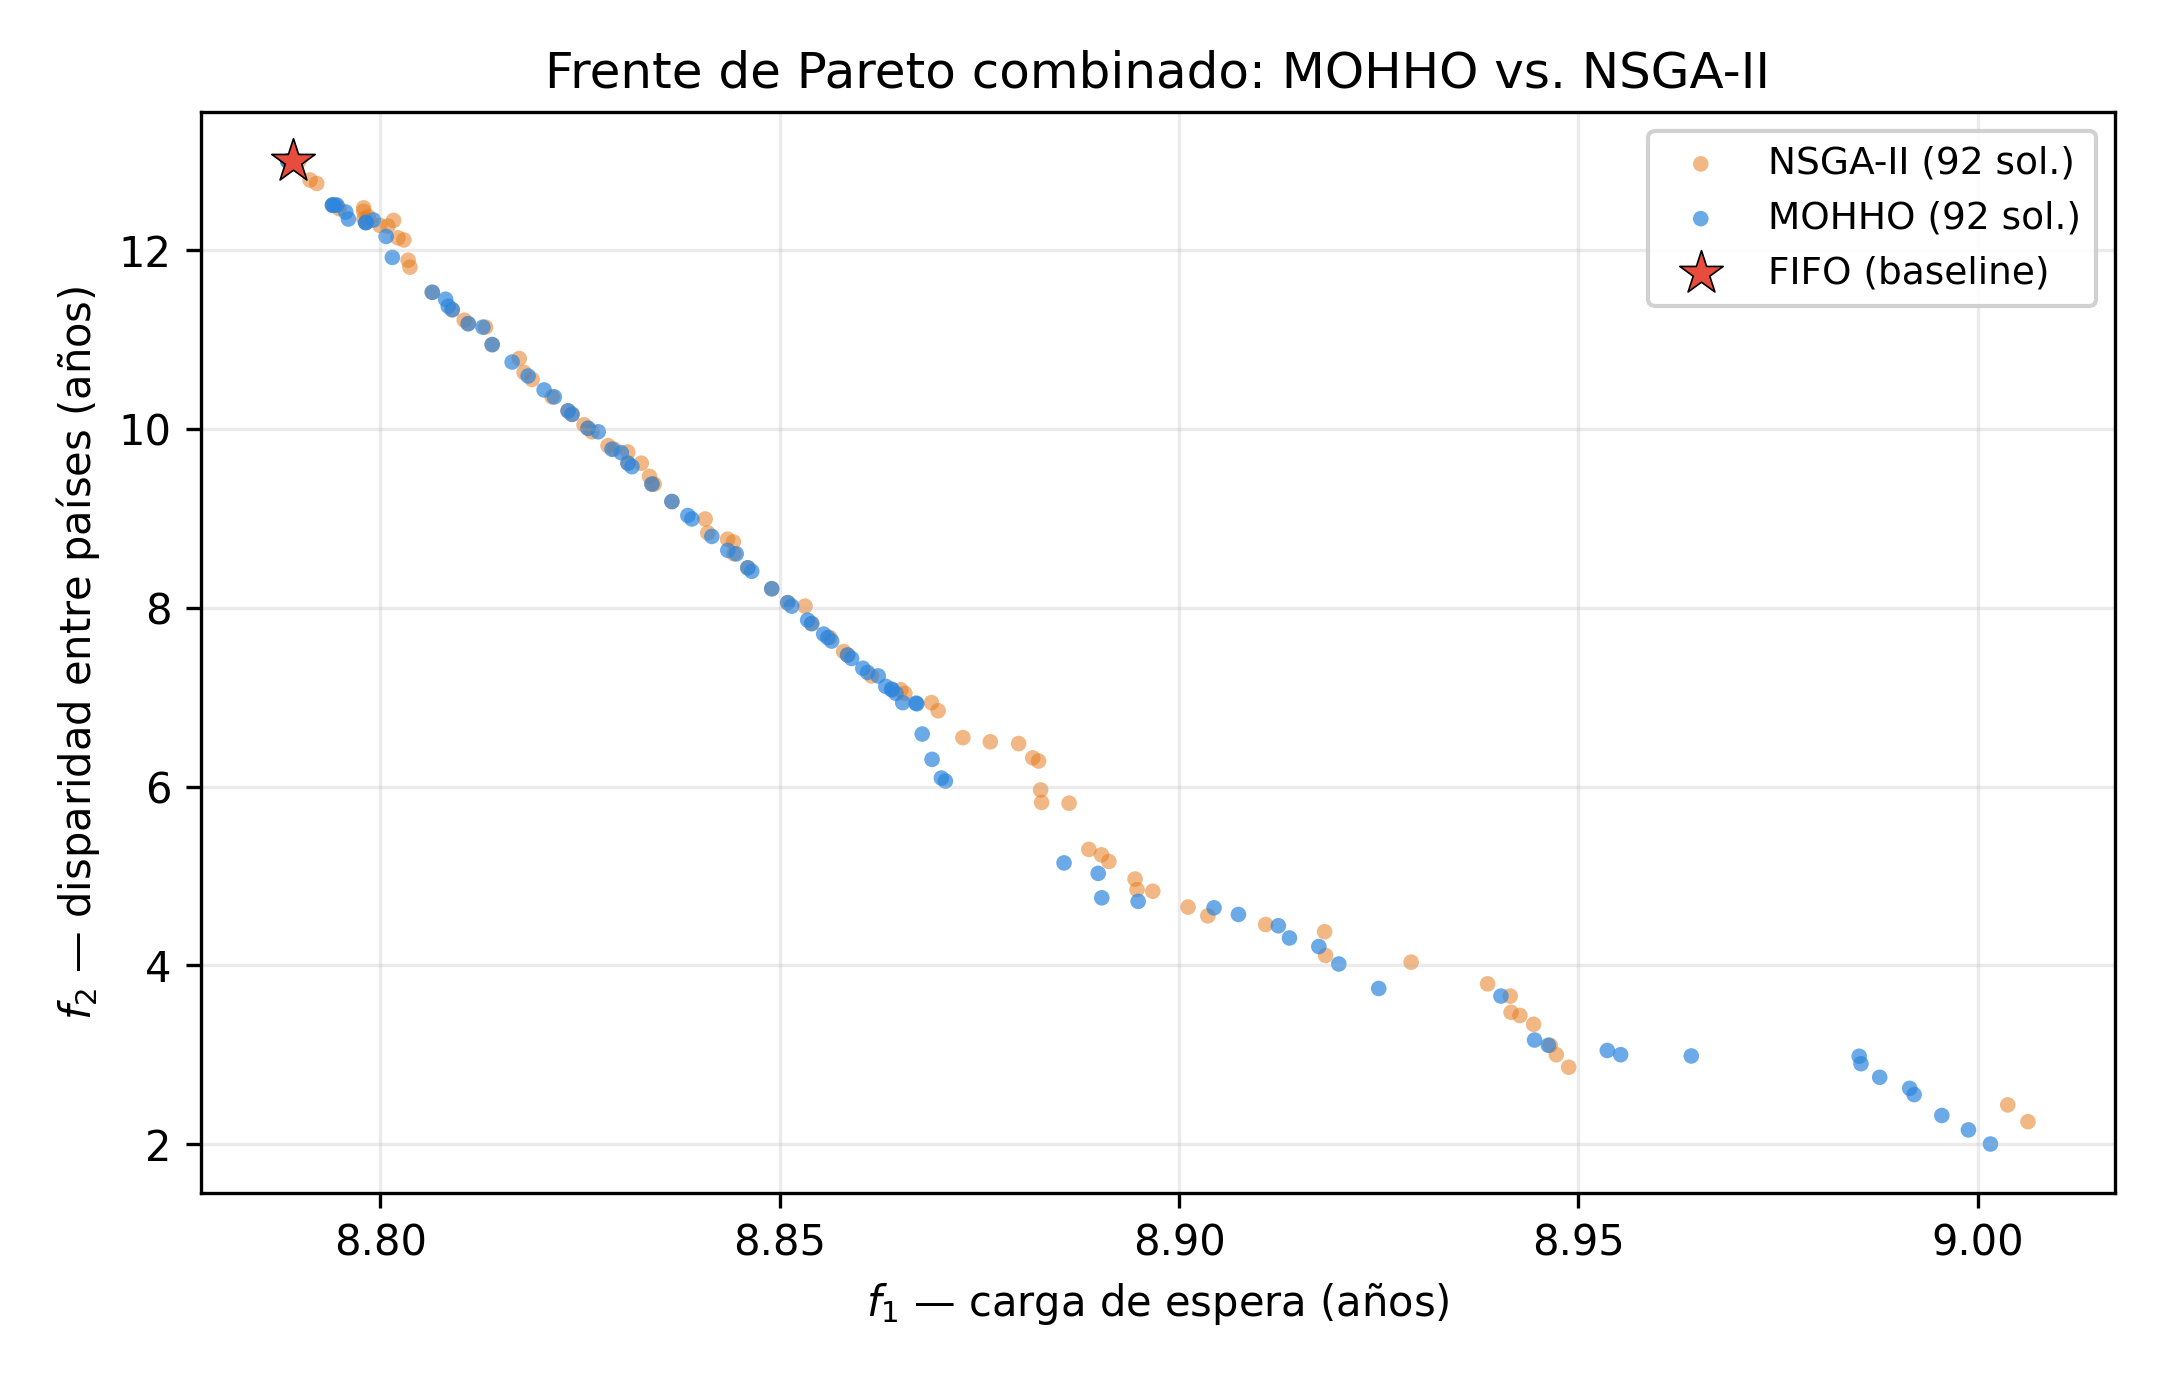
\includegraphics[width=0.92\textwidth]{nsga2_comparison.png}
    \caption{Frente de Pareto combinado de MOHHO (azul, 406 soluciones) frente al de NSGA-II (naranja, 173) en la proyección $f_1$--$f_2$. MOHHO cubre el frente con mayor densidad y alcanza regiones de menor $f_1$ que NSGA-II no recupera. El FIFO (estrella roja) es dominado por ambos.}
    \label{fig:nsga2}
\end{figure}

\begin{answerbox}
\textbf{MOHHO supera a NSGA-II en todas las métricas.} Obtiene mayor hipervolumen medio ($+7.2\%$) con \textbf{menor variabilidad} (CV $1.56\%$ vs.\ $2.84\%$). La ventaja es \textbf{estadísticamente significativa}: prueba U de Mann-Whitney unilateral sobre las 30 corridas, $p\approx1.6\times10^{-10}$, con tamaño de efecto $A_{12}=0.97$ (grande: MOHHO supera a NSGA-II en el $97\%$ de las comparaciones por pares). Además converge mucho mejor (IGD $7.4\times$ menor), distribuye las soluciones de forma más uniforme (menor \textit{spacing}) y recupera $2.3\times$ más soluciones no dominadas. La causa principal es el \textbf{archivo externo con poda por \textit{crowding distance}} de MOHHO, que acumula y preserva diversidad sin el límite del tamaño de población que restringe a NSGA-II a $\leq 50$ soluciones por corrida, sumado al balance exploración--explotación gobernado por la energía $E(t)$. NSGA-II sigue siendo competitivo (domina ampliamente al FIFO), pero MOHHO es la mejor opción para este problema.
\end{answerbox}

\subsection{Escenarios de política y entregable al usuario}
\label{sec:escenarios}
El frente de Pareto no impone una sola respuesta: ofrece un \textbf{menú de políticas}. La plataforma traduce el frente en \textbf{cinco escenarios} accionables, cada uno priorizando un objetivo distinto: \textit{Humanitario} (mínima espera, $f_1$), \textit{Equidad} (mínima disparidad, $f_2$), \textit{Máxima utilización} (cero desperdicio, $f_3$), \textit{Equilibrio} (punto de rodilla del frente) y el \textit{FIFO} actual como referencia. La Figura~\ref{fig:scenarios} compara su perfil: cada escenario sobresale en su objetivo, mientras que el FIFO queda como una figura delgada (dominada en equidad y utilización).

\begin{figure}[htbp]
    \centering
    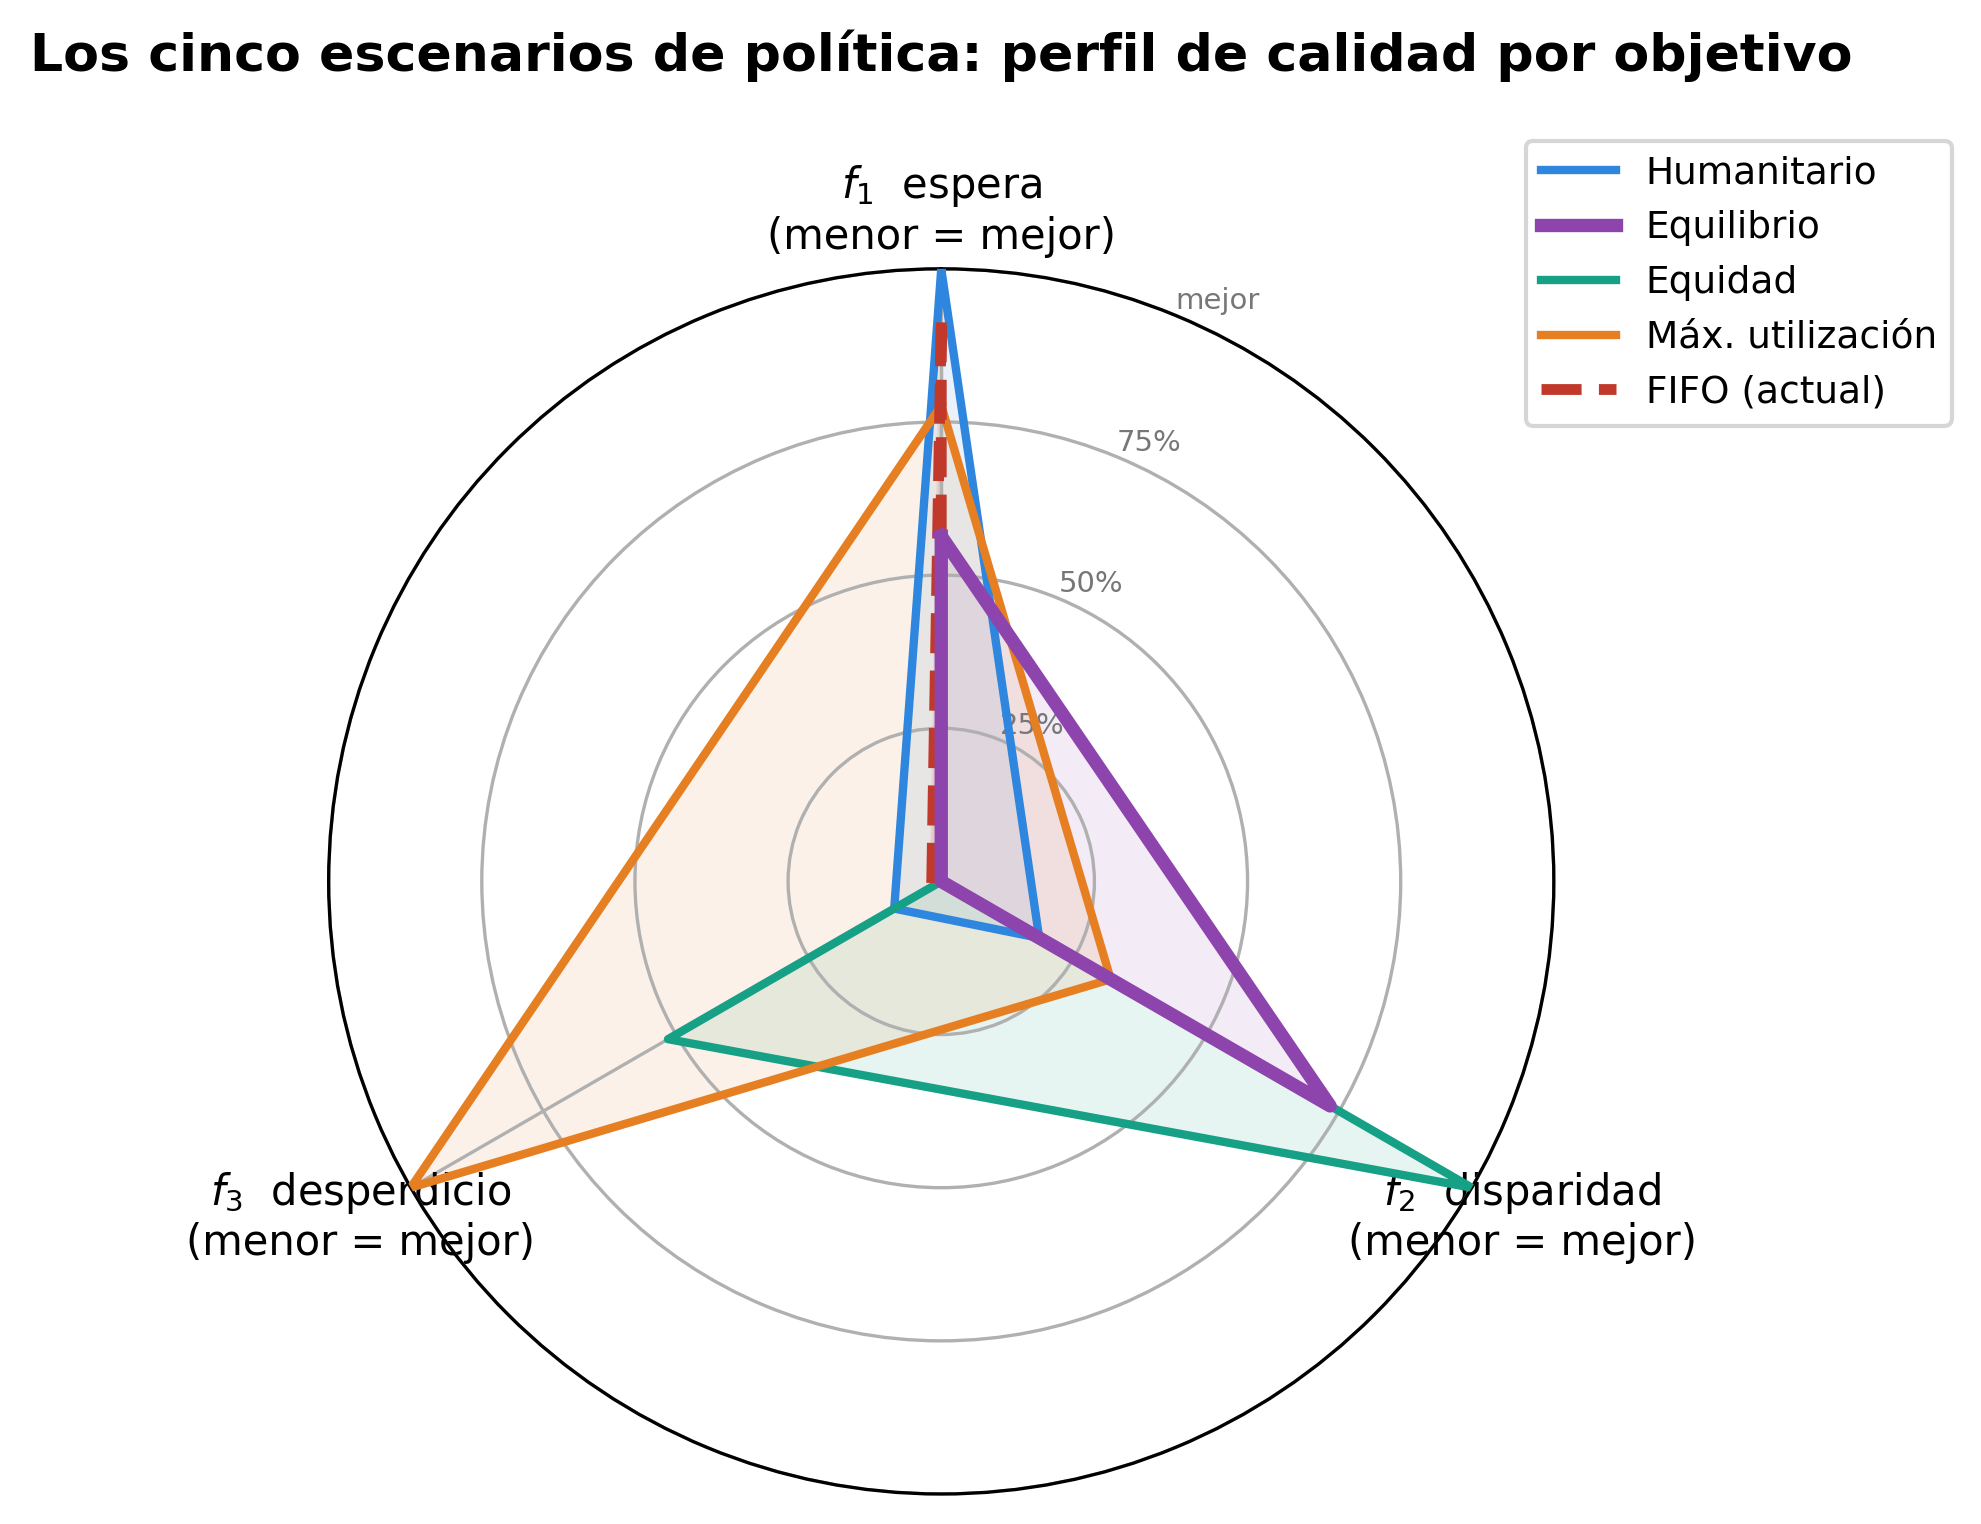
\includegraphics[width=0.90\textwidth]{fig_scenarios.png}
    \caption{Perfil de calidad de los cinco escenarios en los tres objetivos (calidad relativa entre escenarios; el borde exterior marca al mejor de los cinco en ese objetivo). Cada política se especializa; el FIFO es la de menor área, confirmando su carácter dominado.}
    \label{fig:scenarios}
\end{figure}

Elegida una política, el \textbf{entregable concreto} para el tomador de decisiones es la \textbf{asignación de visas por país}. La Figura~\ref{fig:entregable} muestra la del escenario \textit{Equilibrio}: una distribución que usa el 100\,\% de las 140{,}000 visas ($f_3=0$) y, frente al FIFO, redistribuye cupo hacia países hoy subatendidos (Filipinas, México, Corea del Sur, Pakistán, Brasil), reduciendo la disparidad de 12.64 a 5.95 años sin penalizar a India y China (ambas en su tope de 25{,}620). Conviene aclarar que este escenario \textit{Equilibrio} (punto de rodilla del frente, $f_3=0$, 140{,}000 visas) y la solución de compromiso de la Figura~\ref{fig:app-deliver} (§\ref{sec:entregable}, 122{,}380 visas) son \emph{dos puntos distintos del mismo frente de Pareto}: el primero prioriza la utilización total, mientras que el segundo es una elección interactiva del explorador. Ambos son válidos; cuál adoptar depende del criterio del tomador de decisiones.

\begin{figure}[htbp]
    \centering
    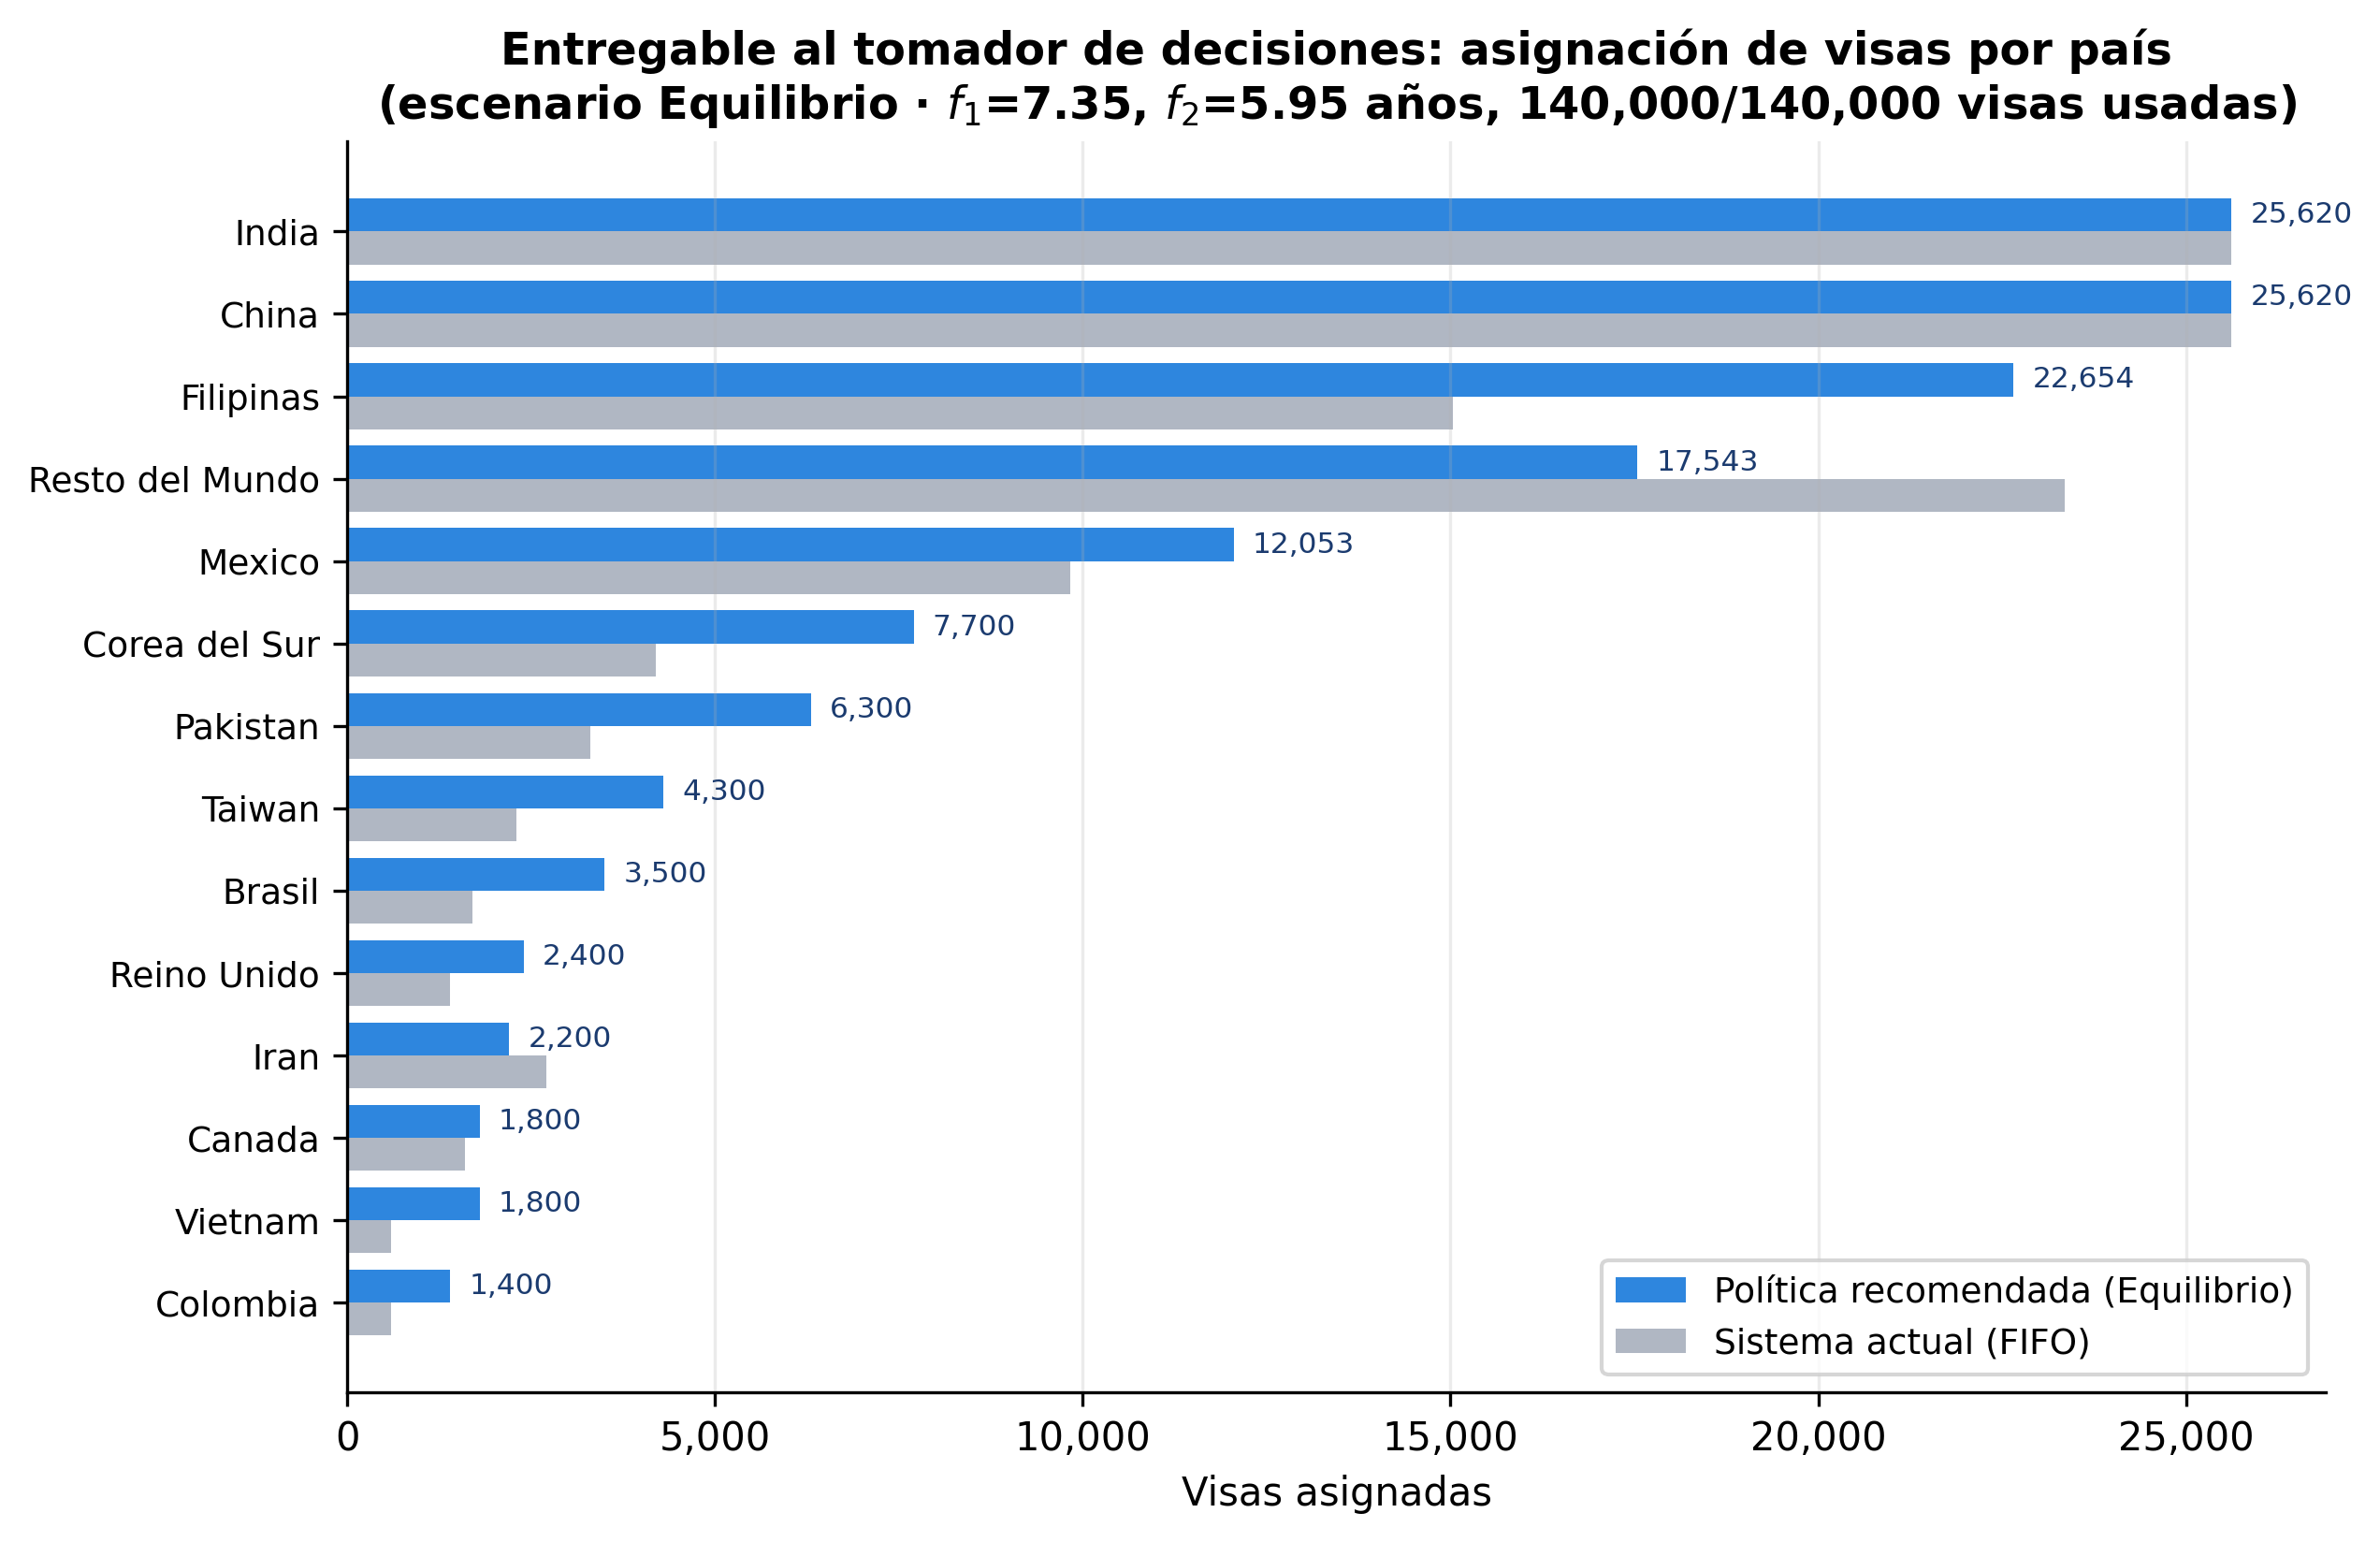
\includegraphics[width=0.97\textwidth]{fig_entregable.png}
    \caption{Entregable final al tomador de decisiones: asignación recomendada de visas por país (escenario \textit{Equilibrio}) frente al sistema FIFO. Es la salida accionable del modelo: una tabla de cuántas visas recibe cada país.}
    \label{fig:entregable}
\end{figure}

% ==========================================================
\section{Interpretación crítica}
\label{sec:critico}

\subsection{Naturaleza del compromiso (trade-off)}
El conflicto entre objetivos es \textbf{estructural}, no un artefacto del modelo. India y China concentran $>$60\,\% de la demanda con esperas de 10--13 años; el tope del 7\,\% impide satisfacerla, de modo que reducir la disparidad ($f_2$) obliga a dejar carga sin atender en esos países ($f_1\uparrow$), y repartir con equidad deja capacidad ociosa en categorías saturadas ($f_3\uparrow$). Las tres soluciones extremas de la Tabla~\ref{tab:extremos} son mutuamente no dominadas: prueba empírica de conflicto genuino en tres dimensiones.

\subsection{Análisis de sensibilidad}
\begin{table}[H]
\centering
\renewcommand{\arraystretch}{1.25}
\small
\begin{tabular}{l>{\raggedright\arraybackslash}p{11cm}}
\toprule
\rowcolor{tablehead}
\textcolor{white}{\textbf{Análisis}} & \textcolor{white}{\textbf{Resultado}}\\
\midrule
Tamaño de archivo & Con $|A|=500$ (sin poda) el frente natural tiene $\sim$211 soluciones/corrida; el HV difiere $<0.03\%$ respecto a $|A|=100$. La poda por \textit{crowding distance} elimina redundancia sin pérdida de calidad.\\
\rowcolor{gray!8}
Iteraciones necesarias & 99\,\% del HV en la iteración 134; las 200 finales aportan $<0.5\%$. $T=500$ es conservador; $T\approx200$ bastaría.\\
Rigidez de $f_1$ & El rango de $f_1$ (0.35 años) es 28$\times$ más estrecho que el de $f_2$. Como la demanda total (868{,}098) excede por mucho las 140{,}000 visas, casi cualquier permutación deja una carga no atendida similar: la variabilidad de $f_1$ es limitada por la estructura del problema, no por el algoritmo.\\
\bottomrule
\end{tabular}
\caption{Análisis de sensibilidad sobre parámetros y estructura del problema.}
\end{table}

\subsection{Fortalezas, limitaciones y mejoras}
\begin{resultbox}
\textbf{Fortalezas.} (1) Factibilidad garantizada por construcción (sin penalizaciones que distorsionen el paisaje de búsqueda). (2) Resultados robustos y reproducibles (CV $1.56\%$). (3) El algoritmo \emph{domina} al sistema vigente. (4) Herramienta web que vuelve el frente navegable y auditable.
\end{resultbox}

\begin{restrictionbox}
\textbf{Limitaciones.} (1) Modelo de un solo año fiscal; ignora efectos intertemporales del backlog. (2) 21 países representativos en lugar de los $\sim$200 reales. (3) La demanda $n_g$ se estima de datos públicos. (4) Se asume que toda visa asignada se utiliza (sin rechazos).
\end{restrictionbox}

\begin{yellowbox}
\textbf{Mejoras futuras.} Extensión multi-periodo ($t\in\mathcal{T}$); ampliación a $\sim$200 países; ampliar la comparación a MOEA/D y SPEA2 (ya se comparó contra NSGA-II, §\ref{sec:nsga2}); validación con datos oficiales desagregados de USCIS.
\end{yellowbox}

\subsection{Implicación de política pública}
El frente de 406 soluciones es un \textbf{mapa cuantificado de compromisos} para el tomador de decisiones: desde priorizar eficiencia ($f_1=7.19$) hasta la equidad radical ($f_2=2.38$) o la utilización total ($f_3=0$). Reducir la disparidad de 12.64 a 2.38 años cuesta solo un 4.1\,\% en $f_1$, lo que indica que mejoras sustanciales de equidad son factibles sin sacrificar eficiencia, resultado coherente con las propuestas de reforma de los topes por país \parencite{fwd2024,crs2023}.

% ==========================================================
\section{Conclusiones}
\label{sec:conclusiones}

\begin{enumerate}\setlength{\itemsep}{2pt}
    \item \textbf{El modelo triobjetivo captura un conflicto real.} Las 406 soluciones no dominadas confirman un compromiso genuino entre eficiencia ($f_1$), equidad ($f_2$) y utilización ($f_3$); las tres soluciones extremas son mutuamente no dominadas.
    \item \textbf{MOHHO supera al FIFO en los tres objetivos.} Existen asignaciones que dominan estrictamente al sistema vigente, que por tanto no es Pareto-óptimo. La utilización total es factible (38 soluciones con $f_3=0$).
    \item \textbf{El algoritmo es robusto y reproducible.} HV $=1{,}785{,}803\pm27{,}831$ (CV $1.56\%$), con convergencia efectiva antes de la iteración 150 de las 500.
    \item \textbf{MOHHO supera a NSGA-II en todas las métricas.} Bajo idéntico problema, codificación y presupuesto, MOHHO logra mayor hipervolumen ($+7.2\%$), menor IGD ($7.4\times$), mejor uniformidad y $2.3\times$ más soluciones no dominadas, con menor variabilidad entre corridas (§\ref{sec:nsga2}).
    \item \textbf{La implementación es correcta y verificable.} La factibilidad se garantiza en el decodificador; la línea base FIFO reproduce exactamente los valores teóricos; y la plataforma web ejecuta, transmite y visualiza el algoritmo real iteración a iteración.
    \item \textbf{El frente de Pareto es una herramienta de decisión.} \textit{Visa Predict AI} convierte un problema de política migratoria en un conjunto navegable de políticas óptimas, cada una con sus consecuencias cuantificadas.
\end{enumerate}

\begin{notebox}
\textbf{Fundamentación técnica.} Este reporte fundamenta teóricamente HHO (energía de escape, exploración/explotación, saltos de Lévy), formaliza el modelo (variables, objetivos, restricciones, dominancia de Pareto), describe los seis operadores y su adaptación multiobjetivo con \textbf{extractos del código real} (Listados~\ref{lst:energia} y \ref{lst:decoder}), y respalda cada afirmación con resultados experimentales reproducibles, una \textbf{comparación rigurosa contra NSGA-II} (§\ref{sec:nsga2}) y su evidencia visual en la plataforma.
\end{notebox}

\bigskip
\begin{center}{\color{uacjyellow}\rule{0.28\linewidth}{1.2pt}}\end{center}
\noindent\textit{Agradecemos al Mtro.~Raúl Gibrán Porras Alaniz su guía y enseñanzas a lo largo del curso, que hicieron posible este proyecto.}

% ===================== REFLEXIONES DEL EQUIPO =====================
\section{Reflexiones del equipo}
\label{sec:equipo}
Cerramos con una reflexión personal de cada integrante sobre lo aprendido al diseñar, implementar y documentar este proyecto.

\begin{tcolorbox}[colback=headerblue!4,colframe=headerblue!45,arc=5pt,boxrule=1pt,left=10pt,right=12pt,top=9pt,bottom=9pt]
\begin{minipage}[c]{3.0cm}\centering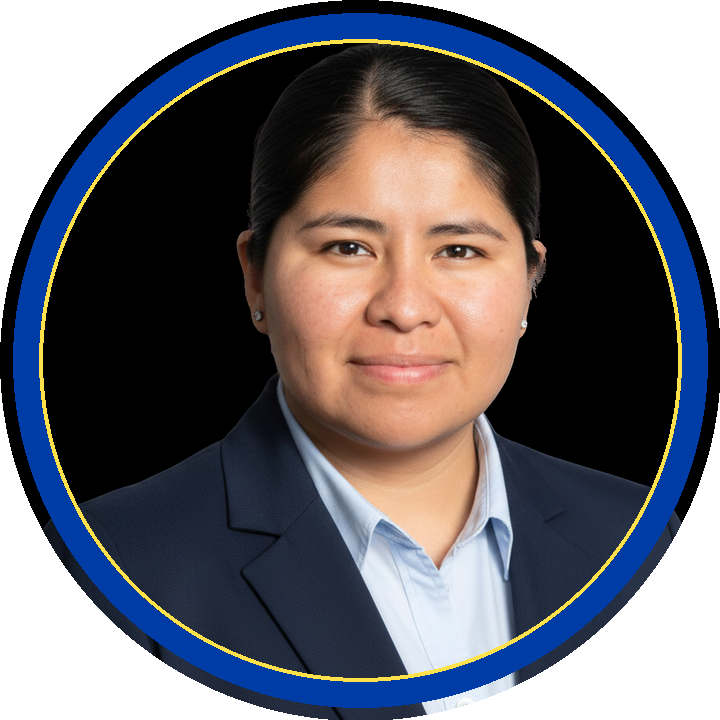
\includegraphics[width=2.8cm]{yazmin_round.png}\end{minipage}\hfill
\begin{minipage}[c]{\dimexpr\linewidth-3.4cm\relax}
{\large\bfseries\color{headerblue} Yazmín Ivonne Flores Martínez}\quad\textcolor{uacjgray}{\small$\bullet$\ 261548}\\[2pt]
{\color{uacjyellow}\rule{0.32\linewidth}{1.6pt}}\\[4pt]
\small\itshape Este proyecto transformó mi manera de ver la optimización: un modelo matemático puede dar voz a un problema profundamente humano. Formular la equidad entre nacionalidades como la función objetivo $f_2$ y verla caer de 12.6 a 2.4 años me mostró que la justicia distributiva es medible y, sobre todo, alcanzable. Aprendí que detrás de cada cifra del \textit{backlog} hay una familia que espera, y que una metaheurística bien planteada puede iluminar políticas más justas.
\end{minipage}
\end{tcolorbox}

\vspace{4pt}
\begin{tcolorbox}[colback=sectiongreen!4,colframe=sectiongreen!45,arc=5pt,boxrule=1pt,left=10pt,right=12pt,top=9pt,bottom=9pt]
\begin{minipage}[c]{3.0cm}\centering
\includegraphics[width=2.8cm]{javi_round.png}\end{minipage}\hfill
\begin{minipage}[c]{\dimexpr\linewidth-3.4cm\relax}
{\large\bfseries\color{headerblue} Javier Augusto Rebull Saucedo}\quad\textcolor{uacjgray}{\small$\bullet$\ 263483}\\[2pt]
{\color{uacjyellow}\rule{0.32\linewidth}{1.6pt}}\\[4pt]
\small\itshape Llevar MOHHO del papel a una plataforma que ejecuta y visualiza cada iteración fue mi mayor aprendizaje: comprendí que la factibilidad se \emph{diseña} en el decodificador, no se castiga con penalizaciones. Validar el algoritmo contra NSGA-II (y verlo ganar en las cuatro métricas con significancia estadística) cerró el círculo entre teoría, implementación y evidencia. La metaheurística dejó de ser una metáfora para volverse ingeniería reproducible.
\end{minipage}
\end{tcolorbox}

% ===================== REFERENCIAS =====================
\printbibliography[title={Referencias}]

\end{document}
